
\documentclass[11pt]{article}
\usepackage{amsmath, amssymb, graphicx, outline, float, cite, color}
\usepackage{lineno}

%%%%%%%%%%%%%%%%%%%%%%%%%%%%%%%%%%%%%%%%%
% Wenneker Article
% Structure Specification File
% Version 1.0 (28/2/17)
%
% This file originates from:
% http://www.LaTeXTemplates.com
%
% Authors:
% Frits Wenneker
% Vel (vel@LaTeXTemplates.com)
%
% License:
% CC BY-NC-SA 3.0 (http://creativecommons.org/licenses/by-nc-sa/3.0/)
%
%%%%%%%%%%%%%%%%%%%%%%%%%%%%%%%%%%%%%%%%%

%----------------------------------------------------------------------------------------
%	PACKAGES AND OTHER DOCUMENT CONFIGURATIONS
%----------------------------------------------------------------------------------------

\usepackage[english]{babel} % English language hyphenation

\usepackage{microtype} % Better typography

\usepackage{amsmath,amsfonts,amsthm} % Math packages for equations

\usepackage[svgnames]{xcolor} % Enabling colors by their 'svgnames'

\usepackage[hang, small, labelfont=bf, up, textfont=it]{caption} % Custom captions under/above tables and figures

\usepackage{booktabs} % Horizontal rules in tables

\usepackage{lastpage} % Used to determine the number of pages in the document (for "Page X of Total")

\usepackage{graphicx} % Required for adding images

\usepackage{enumitem} % Required for customising lists
\setlist{noitemsep} % Remove spacing between bullet/numbered list elements

\usepackage{sectsty} % Enables custom section titles
\allsectionsfont{\usefont{OT1}{phv}{b}{n}} % Change the font of all section commands (Helvetica)

%----------------------------------------------------------------------------------------
%	MARGINS AND SPACING
%----------------------------------------------------------------------------------------

\usepackage{geometry} % Required for adjusting page dimensions

\geometry{
	top=2cm, % Top margin
	bottom=2cm, % Bottom margin
	left=3cm, % Left margin
	right=3cm, % Right margin
	includehead, % Include space for a header
	includefoot, % Include space for a footer
	%showframe, % Uncomment to show how the type block is set on the page
}

\setlength{\columnsep}{7mm} % Column separation width

%----------------------------------------------------------------------------------------
%	FONTS
%----------------------------------------------------------------------------------------

\usepackage[T1]{fontenc} % Output font encoding for international characters
\usepackage[utf8]{inputenc} % Required for inputting international characters

\usepackage{XCharter} % Use the XCharter font

%----------------------------------------------------------------------------------------
%	HEADERS AND FOOTERS
%----------------------------------------------------------------------------------------

\usepackage{fancyhdr} % Needed to define custom headers/footers
\pagestyle{fancy} % Enables the custom headers/footers

\renewcommand{\headrulewidth}{0.0pt} % No header rule
\renewcommand{\footrulewidth}{0.4pt} % Thin footer rule

\renewcommand{\sectionmark}[1]{\markboth{#1}{}} % Removes the section number from the header when \leftmark is used

%\nouppercase\leftmark % Add this to one of the lines below if you want a section title in the header/footer

% Headers
\lhead{} % Left header
\chead{\textit{\thetitle}} % Center header - currently printing the article title
\rhead{} % Right header

% Footers
\lfoot{} % Left footer
\cfoot{} % Center footer
\rfoot{\footnotesize Page \thepage\ of \pageref{LastPage}} % Right footer, "Page 1 of 2"

\fancypagestyle{firstpage}{ % Page style for the first page with the title
	\fancyhf{}
	\renewcommand{\footrulewidth}{0pt} % Suppress footer rule
}

%----------------------------------------------------------------------------------------
%	TITLE SECTION
%----------------------------------------------------------------------------------------

\newcommand{\authorstyle}[1]{{\large\usefont{OT1}{phv}{b}{n}\color{DarkRed}#1}} % Authors style (Helvetica)

\newcommand{\institution}[1]{{\footnotesize\usefont{OT1}{phv}{m}{sl}\color{Black}#1}} % Institutions style (Helvetica)

\usepackage{titling} % Allows custom title configuration


%\newcommand{\HorRule}{\color{DarkGrey}\rule{\linewidth}{1pt}} % Defines the gold horizontal rule
\newcommand{\HorRule}{\color{DarkGoldenrod}\rule{\linewidth}{1pt}} % Defines the gold horizontal rule
 
\pretitle{
	\vspace{-30pt} % Move the entire title section up
	\HorRule\vspace{10pt} % Horizontal rule before the title
	\fontsize{20}{18}\usefont{OT1}{phv}{b}{n}\selectfont % Helvetica
	\color{DarkRed} % Text colour for the title and author(s)
}

\posttitle{\par\vskip 15pt} % Whitespace under the title

\preauthor{} % Anything that will appear before \author is printed

\postauthor{ % Anything that will appear after \author is printed
	\vspace{10pt} % Space before the rule
	\par\HorRule % Horizontal rule after the title
	\vspace{20pt} % Space after the title section
}

%----------------------------------------------------------------------------------------
%	ABSTRACT
%----------------------------------------------------------------------------------------

\usepackage{lettrine} % Package to accentuate the first letter of the text (lettrine)
\usepackage{fix-cm}	% Fixes the height of the lettrine

\newcommand{\initial}[1]{ % Defines the command and style for the lettrine
	\lettrine[lines=3,findent=4pt,nindent=0pt]{% Lettrine takes up 3 lines, the text to the right of it is indented 4pt and further indenting of lines 2+ is stopped
		%\color{DarkRed}% Lettrine colour
		\color{DarkGoldenrod}% Lettrine colour
		{#1}% The letter
	}{}%
}

\usepackage{xstring} % Required for string manipulation

\newcommand{\lettrineabstract}[1]{
	\StrLeft{#1}{1}[\firstletter] % Capture the first letter of the abstract for the lettrine
	\initial{\firstletter}\textbf{\StrGobbleLeft{#1}{1}} % Print the abstract with the first letter as a lettrine and the rest in bold
}

%----------------------------------------------------------------------------------------
%	BIBLIOGRAPHY
%----------------------------------------------------------------------------------------

%\usepackage[backend=bibtex,style=authoryear,natbib=true]{biblatex} % Use the bibtex backend with the authoryear citation style (which resembles APA)

%\addbibresource{example.bib} % The filename of the bibliography

%\usepackage[autostyle=true]{csquotes} % Required to generate language-dependent quotes in the bibliography



\graphicspath{ {Figs/} }

\usepackage[normalem]{ulem}
\usepackage[T1]{fontenc}
\usepackage[utf8]{inputenc}
\usepackage{authblk}

\newcommand{\tcr} { \textcolor{red} }
\newcommand{\tcb} { \textcolor{blue} }


\title{
Modeling the competing effects of the immune system and EMT on epithelial cancers
}

\author{Daniel R. Bergman$^{1}$,
Matthew Karikomi\,$^{1}$,
Qing Nie\,$^{1,2,*}$
and Adam L. MacLean\,$^{3,*}$
}
\affil{
  $^1$Department of Mathematics, University of California, Irvine,  Irvine, CA 92697, USA \\
  $^2$Department of Cell and Developmental Biology, University of California, Irvine, Irvine, CA 92697, USA \\
  $^3$Department of Biological Sciences, University of Southern California, Los Angeles, CA 90089, USA \\
  $^*$Correspondence:  qnie@uci.edu (QN); macleana@usc.edu (ALM).
}

\renewcommand\Authands{ and }

\date{}


\begin{document}
\maketitle


\section*{Abstract}
\sout{Preceding and d}\tcb{D}uring cancer progression, the immune system is engaged in complex sets of interactions with epithelia that affect tumor \sout{incidence and} prognosis.
Inflammation also has significant effects on gastrointestinal and pancreatic tumors.
Moreover, epithelial cell plasticity can significantly alter disease trajectories (for better or worse) via epithelial-to-mesenchymal transition (EMT).
Several of the same pathways that regulate EMT are involved in tumor-immune interactions, yet little is known about the mechanisms and consequences of these regulatory processes.
Here we introduce a multiscale evolutionary model to describe the interplay between tumor-immune-EMT interactions and their impact on epithelial tissues.
Through {\em in silico} analysis of large patient cohorts, we found controllable regimes that maximize cancer-free survival.
Delaying \sout{tumorigenesis} \tcb{progression} depended crucially on properties of the mesenchymal phenotype: its growth rate and its immune-evasiveness.
We performed analysis of pancreatic cancer data from The Cancer Genome Atlas to compare clinical measurements with model predictions.
We found, in broad agreement with the model, that association with EMT worsened the survival probabilities of inflammation-associated cancer.
These results offer novel means to delay disease \sout{onset} \tcb{progression} by regulating properties of EMT, and demonstrate the importance of studying cancer-immune interactions in light of EMT.

\linenumbers

%%%%%%%%%%%%%%%%%%%%%%%
%                    INTRODUCTION                    %
%%%%%%%%%%%%%%%%%%%%%%%


\section{Introduction}
Cancer and the immune system interact in myriad ways. Beyond direct tumor-immune cell interactions, the immune system modulates the tumor microenvironment (TME): responding to local inflammatory signals, targeting mutated cells, and eradicating tumor cells to potentially restore homeostasis in a local context \cite{de2006paradoxical}. Recent breakthroughs in the field of immunotherapy are beginning to produce therapies that have had a significant impact on patient health and survival \cite{pardoll2012blockade,restifo2012adoptive}.
\par 
Tumor cells interact with the immune system by initiating a sequence of events that results in the activation of the adaptive immune response. This is accomplished by the presentation of antigens recognized by innate immune cells that are transported to lymph nodes where T cells (and other components) can be activated \cite{schreiber11_cancer}. The tumor also engages in cellular processes that indirectly shape the TME, for example by releasing transforming growth factor beta (TGF-$\beta$), thus shifting the TME towards a tumor-supportive environment by enhancing immunosuppression via activation of T regulatory cells (Tregs) \cite{schreiber11_cancer}.
\par
The effects of the immune system on a tumor can be broadly summarized into two modules. The cytotoxic branch of the immune system, such as natural killer cells (NKs) and cytotoxic T cells (CTLs), seek out and lyse tumor cells.
Upon carrying out their effector functions, these cytotoxic cells lose efficacy or deactivate entirely \cite{finn12_immunooncology-1}.
The regulatory branch of the immune system (Tregs and other factors), inhibits the effective functioning of the cytotoxic branch \cite{ruffell2010lymphocytes}.
% Does the following sentence still fit with our new focus on progression? I'm looking specifically at the words "pre-cancerous" and "tumorigenesis".
\tcr{In addition, the immune system plays important regulatory roles in pre-cancerous tissue, where inflammation can increase the probability of tumorigenesis (and/or decrease the time to cancer), \sout{particularly} \tcb{including} in tumors originating in gastrointestinal and pancreatic tissues \cite{hu10_inflammationinduced, balkwill01_inflammation}.}
% Similar concern to above as Guo's paper dealt with initiation, not progression.
\tcr{Recent work raises some questions about the relationship between inflammation and cancer, suggesting that under certain conditions inflammation may not be oncogenic but rather onco-protective \cite{guo17_multiscale}.}
\par
Epithelial-to-mesenchymal transition (EMT) describes a reversible process by which cells with an epithelial phenotype transition into cells with a mesenchymal phenotype.
While epithelial cells are in part defined by their adhesion to neighbors, mesenchymal cells show much greater ranges of motility, and may display stem-like properties \cite{nieto2016emt}, although controversy regarding `stemness' and EMT remains \cite{nie18_stem, sha19_intermediate}.  
Recent work has shown that -- rather than being a binary process -- at least two stable intermediate states exist on the EMT axis \cite{hong2015ovol2, jolly15_coupling}.
Ongoing investigations into the plasticity and stability of EMT overlap with discussions elsewhere, e.g. of discrete vs. continuous processes during cell differentiation \cite{moris16_transition}.
Intermediate states have emerged as a central mechanism by which cell fates (and the noise inherent within them) can be controlled \cite{maclean18_exploring, ta16_controlling, rackauckas18_meanindependent}. 
\par 
% Should we even mention initiation here? Make sure to combine below end-of-sentence refs into single \cite command.
While EMT has for some time been assumed to impact metastasis, more recently EMT-related phenotypes have been linked to other aspects of both tumor \tcr{initiation} \tcb{\cite{puisieux2014oncogenic}} and progression \cite{nieto2016emt}\tcb{\cite{peinado2007snail}}.
TGF-$\beta$ is a master regulator of EMT \cite{lim2012epithelial}, linking it to the signaling networks involved in tumor-mediated immune responses, since Tregs release TGF-$\beta$ upon arriving at the tumor site\cite{terry2017new}. 
\tcb{There is evidence directly linking Treg-secreted TGF-$\beta$ with EMT in hepatocellular carcinoma\cite{shi2019cd4+}.} Thus, even by considering only a single signaling factor, we find these three components (the tumor, the immune system, and EMT) to be linked. It therefore strikes us as a priority to develop models to understand how interactions between each of these three components affect cancer incidence and progression.
\par
Two features of the mesenchymal phenotype are of particular relevance in the context of cancer and the immune system: i) mesenchymal cells are less susceptible to immune clearance \cite{terry2017new}; and ii) mesenchymal cells proliferate on average at a slower rate than epithelial cells.
The immune evasiveness of mesenchymal cells is well-established: as a cell is targeted by cytotoxic immune cells for clearance, a physical connection between the two cells must be established before the lysing event.
This immunological synapse is dependent upon the surface proteins, such as the T-cell receptors of the major histocompatibility complex, of the target cell, and in the case of mesenchymal cells there is preliminary evidence that these surface markers are down-regulated in such a way that the immune synapse is more difficult to form \cite{terry2017new}.
Below we refer to this phenotype as mesenchymal immune evasion (MIE).
\par
The other facet of mesenchymal cells is their slower proliferation rate, and this is tied to the observation that mesenchymal cells have been speculate to exhibit a more ``stemness'' phenotype.
While many cell behaviors are associated with stemness, here we target the specific reduction in proliferation rate \cite{woods2014effects} \sout{(which, under certain conditions can be called quiescence, though we avoid this term as it can be controversial, and is not a necessary assumption to the model developed below)}.
Cancer cells are of course characterized by some degree of unregulated proliferation, thus it is appealing to explore the effects of differential proliferation rates within the cancer cell population.
In our model, we refer to the reduced proliferative capacity associated with a mesenchymal cell phenotype as mesenchymal growth arrest (MGA).
\par
Mathematical oncology, that is, mathematical models of cancer incidence, progression, and treatment, has become a well-developed field; many models have offered insight into the cellular interactions underlying cancer and its interplay with the immune system, including classic \cite{anderson98_continuous, sherrattjonathana.92_oncogenes, pillis05_validated} and more recent works \cite{kim18_cell, gallaher14_bridging, gallaher18_spatial, an15_agentbased, serre16_mathematical, louzoun14_mathematical, briones-orta13_arkadia, lavi13_role, greene15_modeling, greene16_mathematical, cho17_modeling-1,  benzekry17_mathematical, owen11_mathematical, west18_multidrug}. These studies have increased our understanding of how tumors grow in the presence of various immune components, and how treatment regimes can be designed to maximize the efficacy of cytotoxicity while minimizing risks to the patient. However, to our knowledge no models have addressed how the effects of EMT alter interactions between the immune system and cancer, and the subsequent implications for treatment. 
\par
Here we develop a model with the goal of studying interactions between the tumor, the immune system and EMT.
We seek to describe a set of crucial molecular and cellular interactions in epithelial tissue cells, including effects due to DNA damage and mutation, to investigate the probability that cancer will \sout{occur} \tcb{progress} and, if so, when.
A recent model of cancer-immune interactions \cite{guo17_multiscale} described the effects of the TME on the risk of cancer, and we build on the core cell cycle component of this model, adding significant new interactions to the immune component of the model (which was previously modeled by a single interaction), as well as adding the effects of EMT.
\tcb{
In doing so, we shift the focus of the previous model from cancer initiation to cancer progression.
We do this to reflect the fact that cancer progression hinges on escape from the immune system and the fact that EMT has a more well-defined role during progression and metastasis.
}
We seek to understand whether this more complex immune module will change our understanding of inflammatory effects on the tumor, and how the epithelial-mesenchymal axis influences these.
\par 
In the next section we develop the model and give explanation of the intuition behind each component.
We then go on to analyze its behavior.
Global sensitivity analysis identifies parameters that are crucial for \sout{tumorigenesis} \tcb{progression}.
We then study these in more depth, focusing on the competing effects of EMT and of the immune system on \sout{tumorigenesis} \tcb{progression}: we find that EMT intricately regulates \sout{tumorigenesis} \tcb{progression} and that under certain regimes a careful balance of EMT- and immune-driven processes can significantly prolong cancer-free survival.
\sout{To test these predictions, we analyze data from the Cancer Genome Atlas (TCGA), and find evidence for the synergistic effects predicted by the model for patients with pancreatic cancer.}
\tcb{To test these predictions, we analyze data from the Cancer Genome Atlas (TCGA), and find evidence for the synergistic effects of inflammation and EMT predicted by the model for patients with pancreatic cancer.}
% Consider rewriting above

%%%%%%%%%%%%%%%%%%%%%%%
%                         METHODS                        %
%%%%%%%%%%%%%%%%%%%%%%%

\begin{table}[H]
\begin{tabular}{|p{\textwidth}|}
\hline
%%%
\tcb{
\begin{itemize}
\item TGF-$\beta$ is well-mixed within the TME
\item All cells are on the same ``clock'', i.e. they all decide at the same time what to do next
\item During a given cell cycle, exactly one event can happen to any one cell: proliferation, apoptosis, immune clearance, or rest
\item All tissue cells (mutated and non-mutated) are equally likely to encounter immune cells
\item Other spatial effects are ignored by the model, e.g. angiogenesis, hypoxia, invasive front, and chemotaxis
\item The initial cells are mutated, but are not able to form an aggressive cancer without further mutations
\end{itemize}
}
\\
\hline
\end{tabular}
\caption{\tcb{Basic assumptions of the model}}
\label{table:model_assumptions}
\end{table}


\section{Methods}
We develop an agent-based model to describe the relationships between cancer, the immune system, and EMT, building on cell-cycle and tissue-cell components of \cite{guo17_multiscale}. 
The agents in the model are the tissue cells \sout{with tumorigenic potential} \tcb{that have already formed a non-aggressive tumor yet have not progressed}.
\sout{These can either be mutation-free or, resulting from DNA damage during the cell cycle, can have any combination of three possible pathway mutations (shown in Fig. \ref{fig:ModelIntro}A).}
\tcb{
In the process of the simulation, these cells can acquire new pathway mutations among three possible (shown in Fig. \ref{fig:ModelIntro}A).
}
If the pathway is mutated, the component is colored red and is marked with `X'.
\sout{A single mutation is sufficient for the cell to be considered as a mutant cell.}
\tcb{
% I'm not a fan of "hypermutated", but I'll use it for now so that a quick replace all can change it later.
We distinguish between cells that have zero of the three pathway mutations and those that have at least one by referring to the latter as hypermutated.
}
\par
We model immune cells as continuous variables, \sout{appropriate since at the level of immune cells it is not necessary to keep track of single cell effects.}
\tcb{
effectively assuming that the TME is well-mixed with regards to the immune infiltrate.
}
The cytokine TGF-$\beta$ is \sout{\tcr{continuous} within the TME, i.e. the system is well-mixed.}
\tcb{
also assumed to be well-mixed in the TME so that all tissue cells have equal access to it.
}
Tissue cells can take on either epithelial or mesenchymal phenotypes in a plastic manner: these phenotypes depend on both the TME and cell-intrinsic factors.
\sout{While the score is continuous, a threshold determines if a given cell is labeled as epithelial or mesenchymal.}
\tcb{While the EMT score is continuous, a threshold determines if a given cell is labeled as epithelial or mesenchymal.}
% Above line replaced
In Fig. \ref{fig:ModelIntro}A, the EMT labeling is given by the \sout{color} \tcb{shade of blue} of the cell.
Even though each cell does have an EMT score on a spectrum of values, only the labeling influences its interactions in the model.

\subsection{Tissue Cells}\label{TissueCells}
The tissue cells at all times have associated with them two important quantities: which combination of mutations they carry and an EMT score.
The model has three pathways that have the potential to mutate over the course of a simulation.
There is a proliferation pathway that when mutated increases the probability of the cell proliferating.
There is an apoptosis pathway that when mutated decreases the probability of the cell undergoing apoptosis.
There is an immune evasion pathway that when mutated decreases the probability that an immune cell can effectively clear the mutated cell.
The EMT score will be exposited in Section \ref{EMT}. 

\subsection{The Immune System}\label{ImmuneSystem}
The immune system is modeled as having three active immune cell types: NKs, CTLs, and Tregs.
% We could justify the immune system not clearing "base" mutated cells by saying the immune surveillance provides a baseline control over these cells accounted for in their apoptosis. Or suggesting that we are interested in immune activity above and beyond the baseline requirement to keep this tumor in check.
The NKs and CTLs act on the system by recognizing \sout{mutated} \tcb{hypermutated} cells and clearing them.
Upon successful clearance, they themselves are then deactivated and removed from the immune population.
Tregs act on the system by suppressing the effector functions of NKs and CTLs, making it less likely they can clear \sout{mutated} \tcb{hypermutated} cells.
In addition to this, Tregs release TGF-$\beta$ which further shapes the TME by pushing tissues cells more towards a mesenchymal phenotype.

\tcb{
\subsection{Inflammation} % How did we not have a section on this before?
We also include an inflammation score that follows a fixed cycling scheme between low and high inflammatory states.
This is to simulate the various changes to the TME that can happen over long periods of time (days and weeks).
For the purpose of the model, we consider low inflammation to be the default state.
When the inflammation switches to high, then a number of the parameters change values to reflect the additional immune activity.
\tcr{See Table 2 in the supplement to see which parameters are changed by the inflammation score changing.} % Table 2 or S2? Change label in supplement?
}

\subsection{EMT}\label{EMT}
Each tissue cell has an EMT score between 0 and 1.
When the score is above a fixed threshold value, the cell is labeled as mesenchymal.
Otherwise, it is below the threshold and labeled as epithelial.
For the purpose of \tcb{parameter values} of the model, a cell in an epithelial state is considered in the base state, and one in a mesenchymal state will have \sout{some} \tcb{a subset} of its parameters updated.
In particular, mesenchymal cells benefit from increased immune evasion but suffer from decreased proliferation.
Note, that because the immune system can only clear \sout{mutated} \tcb{hypermutated} cells, the increased immune evasion only benefits \sout{mutated} \tcb{hypermutated} mesenchymal cells.
\par
\tcb{
In modeling EMT this way, we are assuming that the same factor, TGF-$\beta$, drives EMT both at initiation and through progression of cancer.
In addition, as per our model assumptions (see Table \ref{table:model_assumptions}), we choose to ignore other factors that are known to induce EMT such as hypoxia as well as the typical spatial organization of epithelial and mesenchymal cells as this pertains to the invasive front.
}
\subsection{Model Simulation}

\subsubsection{Initial conditions} 
Every model run starts with \sout{a fixed amount} \tcb{an amount} of \tcb{tissue} cells, $N_0$ \tcb{, determined by the set of parameters used for the run.
A set of warmup cycles are run to ensure arrival to this steady state.
During these warmup cycles, no mutations are allowed to occur the only immune cells present are NKs.}
\sout{However, different parameter values will lead to different steady states for the population of tissue cells.}
\sout{In light of this, a warmup period of ~1000 cell cycles is used in which time no mutations are allowed to happen.}
\sout{Thus, the only immune cell present is NKs.}
After the warmup cycles are complete, a mutagenic event is simulated in which all the tissue cells experience a random increase in their probability to mutate.
From then on, a cell which proliferates also either mutates or increases its probability of mutating later on.

\subsubsection{Tissue cell fate}
During each cell cycle, every cell randomly is assigned a cell fate from the following options:
\begin{itemize}
\item proliferation
\item apoptosis
\item immune clearance (by NKs or CTLs)
\item rest in $G_0$
\end{itemize}

For each cell, a weight is chosen for each option and these are normalized to probabilities which then are used to randomly determine what each cell does during the cell cycle.

\paragraph{Proliferation}
There are four factors that contribute to the weight of a cell to proliferate.
The first is a base proliferation rate that all cells have, $p$.
Second, if the cell has a mutation in the proliferation pathway ($\delta_P=1$), then the weight for proliferation is proportionally increased by $\Delta_P$.
Third, if the cell is mesenchymal ($\zeta=1$), then the weight for proliferation is proportionally decreased by $\Delta_{\text{MGA}}$, which stands for mesenchymal growth arrest.
% Add: 
\tcb{This lost proliferation for mesenchymal cells will later be used to increase their chance of resting.}
Fourth, there is a negative feedback of the cells on their own proliferation which is quantified by a Hill factor as a function of the tissue cell population, $N_C$, with EC50 term $K_0$.
In total, the weight for proliferation is given by

\begin{equation}\tag{2.1}
\rho_P = p(1+\delta_{P}\Delta_P)(1-\zeta \Delta_{\text{MGA}})\frac{K_0}{K_0+N_C}
\end{equation}

\paragraph{Apoptosis}
There are two factors that contribute to a cell's weight for undergoing apoptosis.
There is a basal apoptosis rate that all cells experience, $d_C$ for death.
Second, if the cell has a mutation in the apoptosis pathway ($\delta_A=1$), then the weight for undergoing apoptosis is proportionally decreased by $\Delta_A$.
In total, the weight for apoptosis is given by 

\begin{equation}\tag{2.2}
\rho_A = d_C(1-\delta_{A}\Delta_A)
\end{equation}

\paragraph{Immune Clearance}
For both NK clearance and CTL clearance, the weights are built with the same factors but have different parameter values for NK and CTLs.
First of all, the cell needs to be \sout{mutated} \tcb{hypermutated} ($\delta_{\text{MUT}}=1$).
Second, there is a Hill factor that captures the probability of an immune cell finding and interacting with the given tissue cell with EC50 term $K_1$.
Third, NKs and CTLs have their own efficacy parameters, $E_{\text{NK}}$ and $E_{\text{CTL}}$, which can be understood as the rate of immune clearance given an immune cell has found the mutated cell.
Fourth, there is a decreasing Hill factor based on the number of Treg cells present with EC50 term $K_2$.
Finally, there are two factors that proportionally decrease the weight of immune clearance depending on if the cell has an immune evasion mutation ($\delta_{\text{IE}}=1$) or if it is mesenchymal ($\zeta=1$) with respective decreases $\Delta_{\text{IE}}$ and $\Delta_{\text{MIE}}$.
In total, the weight of NK clearance is given by

\begin{equation}\tag{2.3}
\rho_{\text{NK}} =\delta_{\text{MUT}} \frac{N_{\text{NK}}}{N_C/K_{1}+N_{\text{NK}}}  \frac{E_{\text{NK}}}{1+N_{\text{Treg}}/K_2} (1-\delta_{\text{IE}}\Delta_{\text{IE}})(1-\zeta \Delta_{\text{MIE}})
\end{equation}

A similar formula holds for CTLs with only the number of CTLs and their efficacy being different from the above equation.


\paragraph{Rest in $G_0$} 
\sout{The weight associated with quiescence is taken as 1 except in the case of mesenchymal cells.
For mesenchymal cells, the weight lost to proliferation is added to the weight of quiescence.
Hence, the weight of quiescence is given by}
\tcb{The weight associated with rest is taken as 1 except in the case of mesenchymal cells.
Recall that mesenchymal cells had their proliferation rate decreased by $1-\zeta\Delta_{\text{MGA}}$ (see Eq. 2.1).
The biological assumption here is that mesenchymal cells instead of proliferating will instead rest, so this lost proliferation weight is added to the resting weight.
Hence, the weight of rest is given by}
% Replace quiescence with rest and explain more above

\begin{equation}\tag{2.4}
\rho_R = 1 + \zeta p(1+\delta_P\Delta_P)\Delta_{\text{MGA}}\frac{K_0}{K_0+N_C}
\end{equation}

\tcb{Again, t}\sout{T}he reason for adding that term is due to the understanding that overall mesenchymal cells proliferate less as individual cells rest longer in the $G_0$ phase.

\subsubsection{Completing the Cell Cycle}
After the cell fates are determined and the results reflected in the system, there are a few things that happen before the system moves on to a new cell cycle.
First, the NK and CTL populations are reduced by the number of mutated cells they cleared.
This represents the fact that individual immune cells lose efficacy as they carry out their effector functions. 
Second, all proliferating cells have a cell-specific probability of undergoing a pathway mutation.
If they do, one is randomly chosen among the three pathways and the pathway in that cell mutates.
If the cell does not undergo a mutation, then its probability of mutation during subsequent cell cycles increases.
\par
Finally, the EMT values for each cell is updated.
This depends on the cells current EMT score and how much TGF-$\beta$ is currently in the system.
% The following sentence could be altered to reflect that the threshold value for $\tau$ is 0, so not only are negative values possible, but very common. So, this is not really so much a TGFB received as it is a change in TGFB signaling.
\sout{Each cell receives an amount of TGF-$\beta$ given by}
\tcb{The amount of TGF-$\beta$ absorbed by all cells is given by an increasing Hill function in terms of the TGF-$\beta$ in the TME.
The saturation effect is to limit the amount of TGF-$\beta$ a cell can absorb in a given time interval.
This quantity is then divided up randomly among the $N_C$ living cells via a normally distributed noise term to determine how much exogenous TGF-$\beta$ each cell receives during this cell cycle.
Should this value, $\tau_i$ in Eq. 2.5, be negative, we interpret this as the cell losing TGF-$\beta$ to the TME and thus being more likely to undergo MET.}

\begin{equation}\tag{2.5}
\tau_i = \frac{\tau_{\text{max}}}{N_C}\frac{\tau/K_3}{1+\tau/K_3} + X_i
, \quad X_i \sim N(0,\sigma^2)
\end{equation}


\tcb{
We then combine $\tau_i$ with the current EMT score of the cell, as a proxy for the endogenous TGF-$\beta$.
Finally, if this quantity is large enough, \sout{the cell undergoes EMT; otherwise, it undergoes MET.} \tcb{the EMT score of the cell increases towards 1; otherwise, it decreases towards 0.}
}
% Need to add better explanation for Hill fn
\sout{The summand on the left deterministically divides up the total TGF-$\beta$ among all $N$ cells evenly and a Hill function on this quantity determines how much TGF-$\beta$ each cell thus receives.}
\sout{Then, some randomness is introduced by the independent and identically distributed variables $X_i$ where $\sigma$ is a parameter in the model.
If this quantity is large enough, relative to the EMT score of the cell, then the cell will undergo EMT and its EMT score will increase.
If not, then the cell undergoes the reverse process, MET, and its EMT score will decrease.
}
Each cell then is relabeled as either epithelial or mesenchymal depending on its new EMT score and whether it is below or above the mesenchymal threshold.
Thus, there are two main factors that determine if a cell will end a cell cycle as mesenchymal: concentration of TGF-$\beta$ in the system and the current EMT score of the cell.

Next, the amount of TGF-$\beta$ for the next cell cycle is determined by the number of mutated cells, $N_{\text{MUT}}$, and the number of Treg cells, $N_{\text{Treg}}$, each one producing a fixed amount of TGF-$\beta$. It is given by

\begin{equation}\tag{2.6}
\tau = \tau_{\text{MUT}}N_{\text{MUT}} + \tau_{\text{Treg}}N_{\text{Treg}}
\end{equation}


Finally, the immune populations are updated.
For the NKs, they obey the following differential equation:
 
\begin{equation}\tag{2.7}
N_{\text{NK}}' = \sigma_{\text{NK}} - d_{\text{NK}}N_{\text{NK}}
\end{equation}

which is discretized to
 
 \begin{equation}\tag{2.8}
N_{\text{NK}}(k+1) = \left (N_{\text{NK}}(k)-\frac{\sigma_{\text{NK}}}{d_{\text{NK}}} \right )\exp(-d_{\text{NK}}\Delta t)+\frac{\sigma_{\text{NK}}}{d_{\text{NK}}}
\end{equation}

For CTLs and Tregs, they rely on \sout{mutant} \tcb{hypermutated} cells being cleared before they can be activated.
Let $N_{\text{MUT}}^*(k)$ represent the number of \sout{mutant} \tcb{hypermutated} cells cleared by the immune system during cell cycle $k$.
In addition, Treg recruitment is upregulated by TGF-$\beta$, which will be incorporated via a Hill function with EC50 term $K_4$.
We choose the following differential equations to govern the CTL and Treg populations:

\begin{equation}\tag{2.9}
\begin{split}
N_\text{CTL}' & = \sigma_{\text{CTL}}N_{\text{MUT}}^* - d_{\text{CTL}}N_\text{CTL} \\
N_\text{Treg}' & = \sigma_{\text{Treg}}N_{\text{MUT}}^* \frac{\tau}{1+\tau/K_4}- d_{\text{Treg}}N_\text{Treg}
\end{split}
\end{equation}

Discretized, these are:

\begin{equation}\tag{2.10}
\begin{split}
N_\text{CTL}(k+1) & =  \left (N_\text{CTL}(k)-\sigma_{\text{CTL}}N_{\text{MUT}}^*(k)/d_{\text{CTL}}\right )\exp(- d_{\text{CTL}}\Delta t) + \sigma_{\text{CTL}}N_{\text{MUT}}^*(k)/d_{\text{CTL}}\\
N_\text{Treg}(k+1) & =  \left (N_\text{Treg}(k)-\frac{\sigma_{\text{Treg}}N_{\text{MUT}}^*(k)}{d_{\text{Treg}}} \frac{\tau(k)}{1+\tau(k)/K_4}\right )\exp(-d_{\text{Treg}}\Delta t)\\
&+ \frac{\sigma_{\text{Treg}}N_{\text{MUT}}^*(k)}{d_{\text{Treg}}} \frac{\tau(k)}{1+\tau(k)/K_4}
\end{split}
\end{equation}

\begin{table}[H]
\begin{center}
 \begin{tabular}{|| c | c||} 
 \hline
 {\bf Name} & {\bf Description}  \\ [0.5ex] 
 \hline
 $p$ & proliferation rate of tissue cells \\ 
 \hline
 $d_C$  & death rate of tissue cells \\
 \hline
$\Delta_\text{MIE}$ &  mesenchymal immune evasion \\
 \hline
 $\Delta_\text{MGA}$ & mesenchymal growth arrest    \\
 \hline
  $\Delta_A$ & \tcr{mutant cells decreased apoptosis}  \\ % should this and the others like it be more clear in stating this is not for all hypermutated cells, but only those with apoptosis pathway mutation?
  \hline
  $\Delta_\text{IE}$ & mutant cells increased immune evasion  \\
  \hline
  $\Delta_P$ & mutant cells increased proliferation  \\
  \hline
 $K_0$ & EC50 term for negative feedback of tissue cells on own proliferation\\
 \hline
 $K_1$ & EC50 term for probability of NK cell finding mutant cell\\
 \hline
  $K_2$ & EC50 term for Treg inhibition of cytotoxic functions  \\
  \hline
  $K_3$ & EC50 term for how much TGF-$\beta$ each cell has \\
  \hline
  $K_4$ & EC50 term for TGF-$\beta$ activation of Tregs \\
  \hline
 $E_\text{NK}$ & rate of NKs clearing mutants  \\
  \hline
  $E_\text{CTL}$ & rate of CTLs clearing mutants \\
  \hline
  $\sigma_\text{NK}$ & NK source rate \\ 
  \hline
  $\sigma_\text{CTL}$ & CTL source rate per cleared \sout{mutant} \tcb{hypermutated} cell \\ 
  \hline
  $\sigma_\text{Treg}$ & Treg source rate per cleared \sout{mutant} \tcb{hypermutated} cell \\ 
  \hline
  $d_\text{NK}$ & NK death rate \\ 
  \hline
  $d_\text{CTL}$ & CTL death rate \\ 
  \hline
  $d_\text{Treg}$ & Treg death rate \\ 
  \hline
  $k_\text{EMT}$ & EMT/MET rate  \\
  \hline
  $\sigma$ & standard deviation of noise in TGF-$\beta$ each cell receives  \\
  \hline
 $\tau_\text{max}$ & max amount of TGF-$\beta$ any cell can receive \\
  \hline 
 $\tau_\text{MUT}$ & rate of TGF-$\beta$ production by mutant cells\\
  \hline
 $\tau_\text{Treg}$ & rate of TGF-$\beta$ production by Treg\\
  \hline
\end{tabular}
  \caption{The model parameter names and descriptions. Note that many of these values are affected by the inflammation state of the system.}
\end{center}
\end{table}

\subsubsection{Mutation and tumorigenesis}
% 3rd Referee did not like this terminology for a tumorigenic event. Should we change it or better explain it?
At the end of each cell cycle, the proportion of tissue cells that are \sout{mutated} \tcb{hypermutated} is calculated, and if it is above a certain threshold, \sout{a tumorigenic event is recorded and the patient is determined to have cancer.}
\tcb{the simulation ends and we declare the tumor to have progressed.}
The Time to Cancer is given as the time from the start of the simulation, not including warmup, until \sout{tumorigenesis.} \tcb{this timepoint.}
Simulations run until either a \sout{tumorigenic event is recorded} \tcb{this occurs} or until the \tcb{predetermined} maximum number of cycles has been reached.

\subsection{Parameter Sensitivity Analysis}
To study parameter sensitivity, we implemented the Morris method, a one-step-at-a-time global sensitivity analysis algorithm.
The algorithm runs the model numerous times by picking several base points and then varying one parameter at a time from each base point and tracking the difference\cite{morris1991factorial, sohier2014improvement}.
Each model run involved 1000 patients and the value returned was the area under the survival curve.
We ran the algorithm by sampling at 30 points in parameter space and then changing each parameter one time at each point.
In the implementation by Sohier, they recommend using at least 10 points\cite{sohier2014improvement}.
\par
To determine which points in parameter space to sample at, we had to create distributions on all parameter values.
To do this, we derived many parameters from existing literature and the rest we made reasoned predictions.
For example, many previous studies have established the parameters of immune population dynamics such as recruitment and death rates\cite{de2014modeling}.
Because our model only works with on the order of $10^2$ tissue cells whereas an actual tumor would have on the order of $10^9$ cells\cite{de2014modeling}, we scaled the parameters so the immune populations would also be proportionately reduced.
That is, for instance, how we ended up with NK cells having a steady state population of 10 cells in the model.
\par
Once we had these parameter values, we created Gaussian distributions centered at these values with large variances and truncated at 0.
Some of the parameters were also truncated to the right because they represented a proportion, such as MIE and MGA, or because we simply wanted to keep the values within a reasonable range, such as the inflammation low and high duration parameters.
The \sout{variances} \tcb{standard deviations} were chosen as twice the mean to get a large spread of values.
\par
% Referee 2 either missed the following line or doesn't understand what average of absolute change means.
\tcr{The algorithm computes the average of the absolute change of the output, which in our model is the area under the survival curve.}
This output of the algorithm, $\mu^*$, is the sensitivity plotted in Fig. \ref{fig:MOAT}.


\subsection{Analysis of patient survival data from TCGA database}
We obtain primary tumor bulk mRNA sequencing and censored survival data for all individuals monitored in the relevant project from the Cancer Genome Atlas (TCGA) from the Genomic Data Commons portal in R, using the package TCGABiolinks.  Given $n >= 1$ gene set keywords (e.g. "inflammatory" and "emt"), the symbolic names of all msigdb gene sets are searched for matches to these keywords, and matched gene sets are grouped by keyword. For each element in the product S of all keyword groups, the following analysis is performed.
\begin{enumerate}
     \item The first principle component of the expression across the gene set is obtained for each element of the n-tuple of gene sets.
     \item Two clusters of n-dimensional patient vectors are obtained by k-means clustering.
     \item The patients are separated by their cluster identity and Kaplan-Meier curves are fit to their corresponding survival data.
     \item Under the null hypothesis that there is no difference between the survival of the two groups, a log-rank test is performed.
     \item The log-rank test p-value for each element in S is placed in an ordered list, the lowest of which defines the element of S whose composite gene sets are most predictive of patient survival in the given TCGA project or tumor type.
\end{enumerate}
Below we analyze data gathered for pancreatic cancer, denoted by ``PAAD'' in TCGA.     

%%%%%%%%%%%%%%%%%%%%%%%
%                          RESULTS                         %
%%%%%%%%%%%%%%%%%%%%%%%

\section{Results}

\subsection{A multiscale agent-based model of EMT-immune-tissue cell interactions to study tumorigenesis}\label{ExplModel}

\begin{figure}
\center
{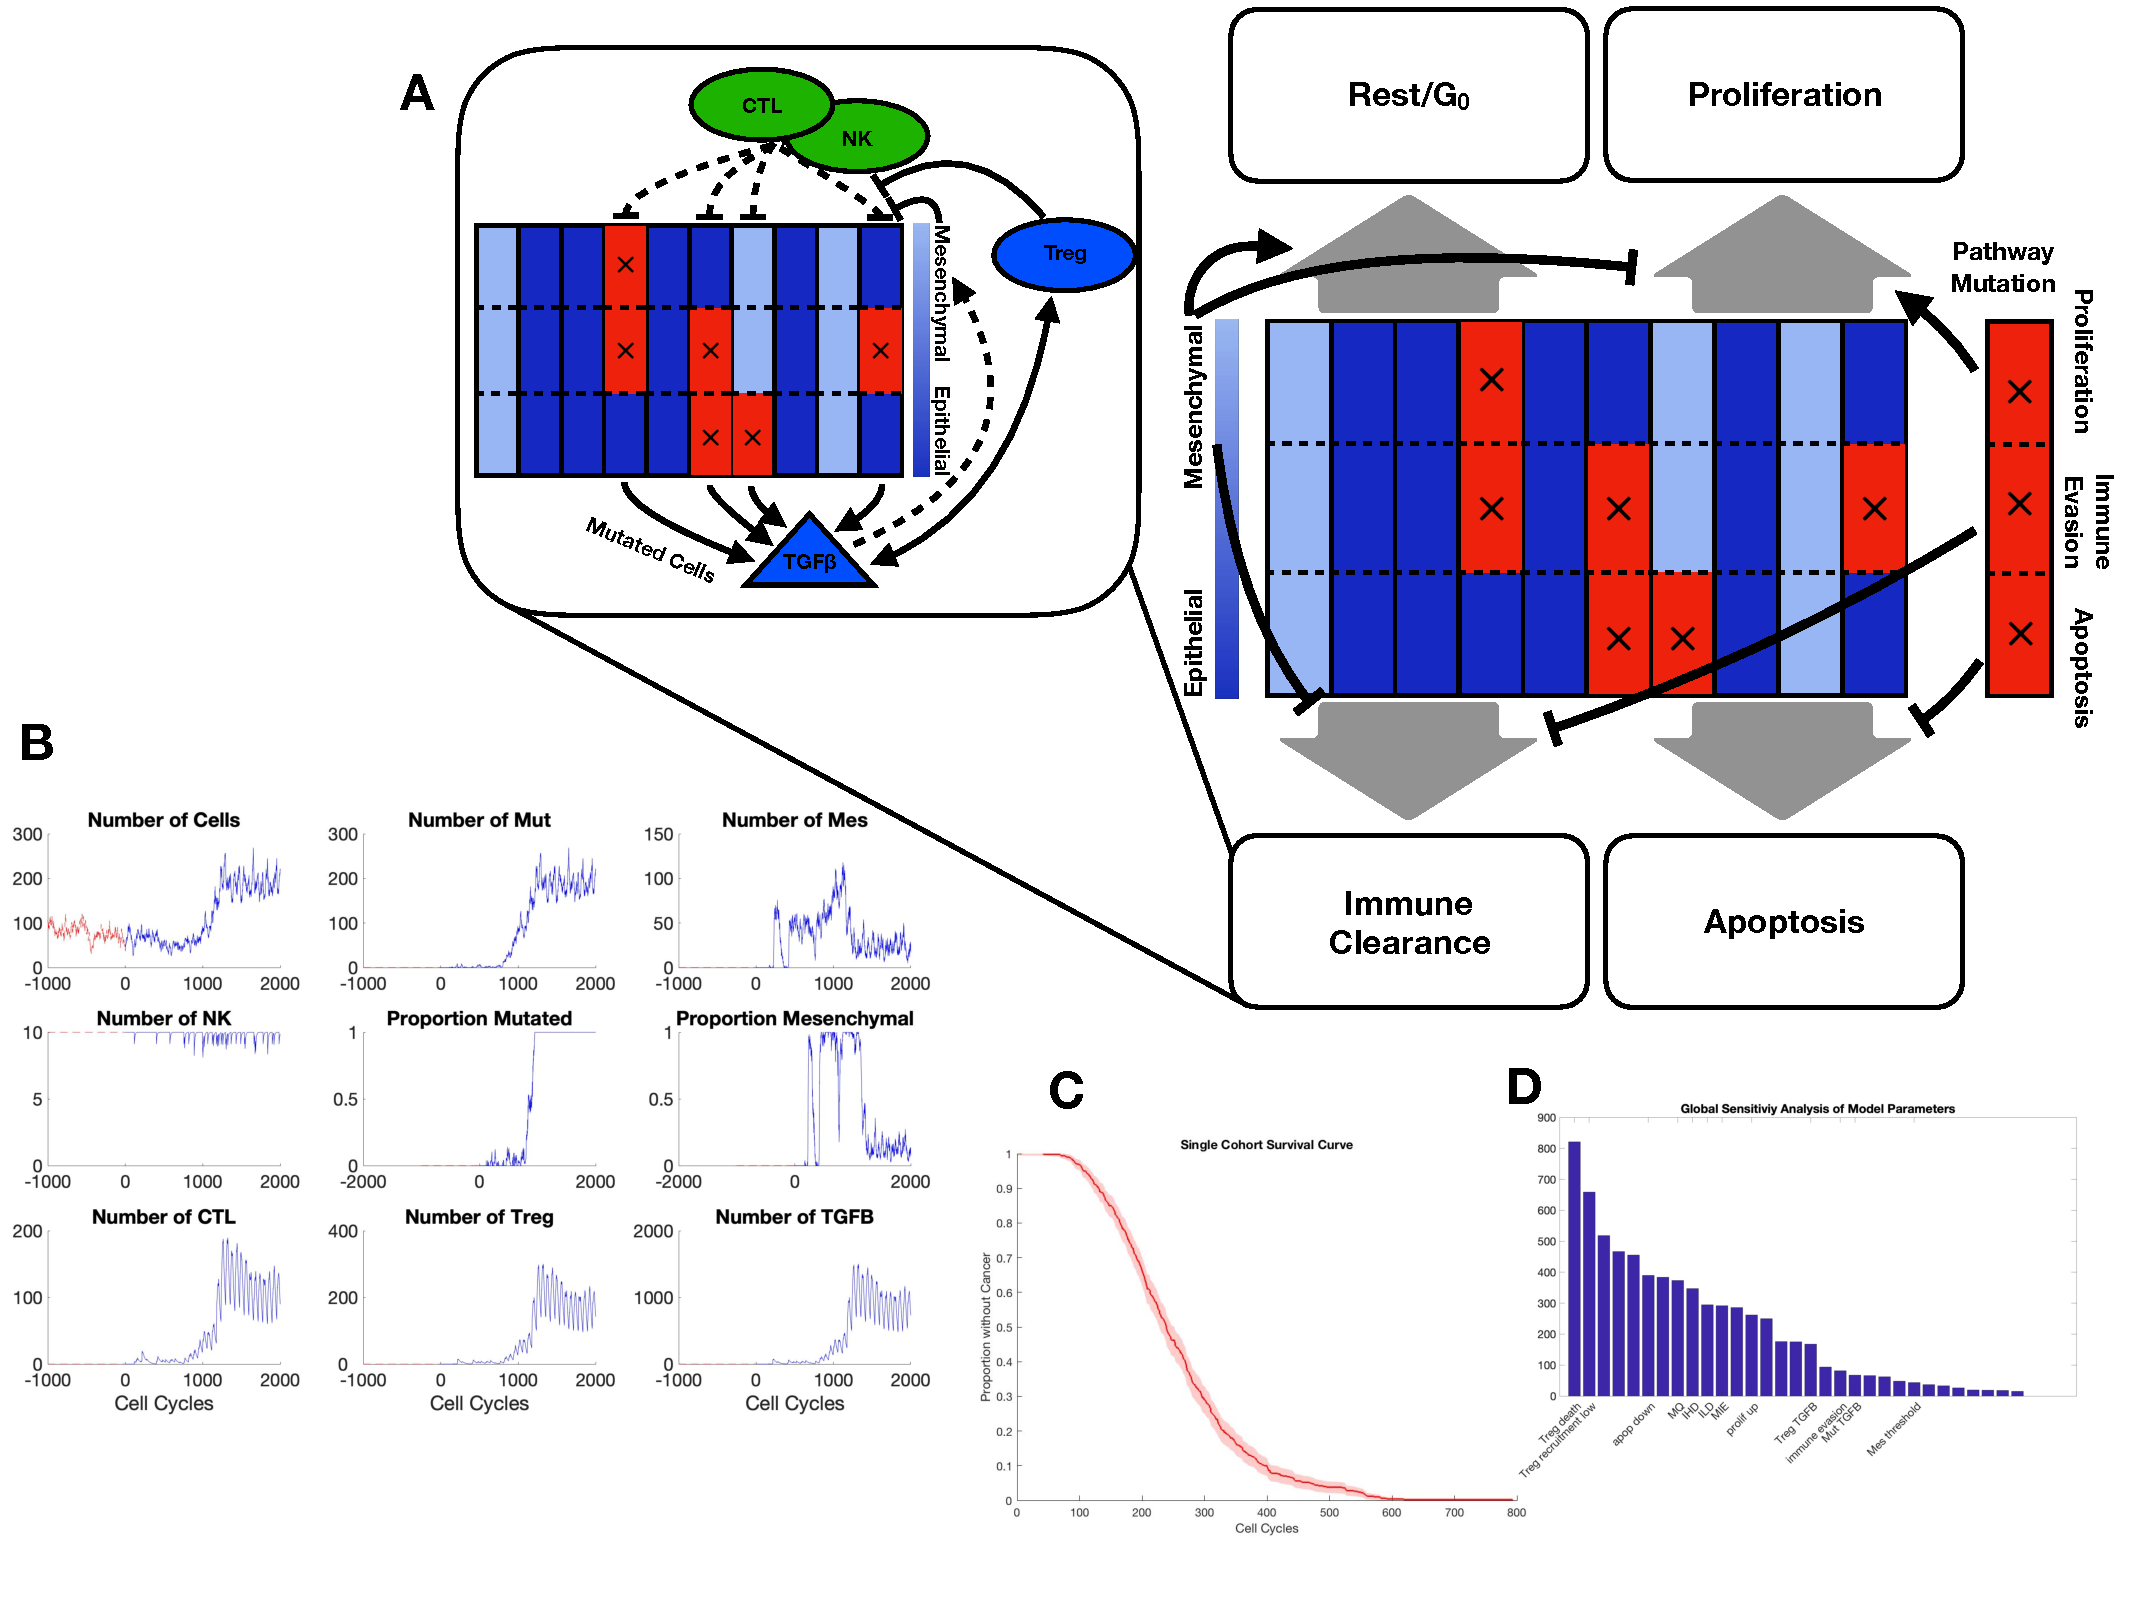
\includegraphics[width=0.9\textwidth]{Figure1/Figure1.pdf}}
\caption{A. Schematic depiction of agent-based model components; \tcb{
each of the 10 columns represents a single tissue cell divided into three compartments representing the state (mutated or not) of the three pathways with mutagenic potential;
}\sout{blue/red denote tissue cells with/without mutations} \tcb{red/blue denotes mutated/unmutated pathways} . Black arrows depict regulation of the cell fate in each cell cycle. Inset depicts major interactions between the immune system and tissue cells.
 %The parameters used in this model can be found in the Supplementary material. Unless otherwise stated, parameter values are assumed to be those found in the Supplement. \tcr{Thoughts on the wording here? Once I have the table, I will use the name of that table.}
B. A representative simulation of one patient. The model parameter values used can be found in Supplementary Table 2. 
The inflammation cycling scheme is represented above the patient dynamics. The vertical dashed line denotes the end of the warmup period. Mut: \sout{mutated} \tcb{hypermutated} cells; Mes: mesenchymal cells. 
C. Survival curve for one cohort of patients with the parameter values given in Supplementary Table 2. }
\label{fig:ModelIntro}
\end{figure}

We begin by investigating general features of the model to establish baseline conditions and to assess the impact of various model components on the key measured outcomes: the \tcr{probability} of cancer, and the Time to Cancer. 
Within the cell cycle, cell fate is determined via a set of rules that are influenced by EMT and immune interactions (Fig. \ref{fig:ModelIntro}A). For example, if a cell undergoes EMT, the probability that it will proliferate is reduced; if a cell gains a mutation in the apoptosis pathway, the probability that it undergoes apoptosis is greatly reduced.
The different means by which the immune system acts on tissue cells are also shown (\ref{fig:ModelIntro}A Inset). NK cells and CTLs attempt to clear \sout{mutated} \tcb{hypermutated} tissue cells, and deactivate upon successfully carrying out their cytotoxic function.
Tregs inhibit cytotoxic activity.
Tregs also release TGF-$\beta$ which promotes the recruitment of Tregs, as well as increasing the rate of EMT.
\par
The inflammation cycling scheme for a typical {\it in silico} patient consists of alternating high and low regimes (Fig. \ref{fig:ModelIntro}B); the inflammation schemes modeled will be discussed in detail in the next section.
For this patient, after the warmup period, cell mutations are observed at a rate low enough that they are cleared by cytotoxic cells before being able to establish a tumor.
\sout{
However, after approximately 1000 cell cycles (750 days), one mutated cell exhibits clonal growth, and a tumor is established.
At this point, large numbers of cells from the adaptive immune system (CTLs and Tregs) are being heavily recruited, and a peak in TGF-$\beta$ expression is observed.
The number of mesenchymal cells increases initially with increasing TGF-$\beta$, but decreases after the clone takes over the tissue.
This shift back towards an epithelial tissue phenotype occurs even though the expression of TGF-$\beta$ remains high.
After 841 cell cycles, the proportion of mutated cells reaches 50\%: this is modeled as the threshold defining tumorigenesis. Thus this patient has a Time to Cancer of 841 cell cycles, or 631 days. 
After cancer incidence, the number of mutated cells continues to grow rapidly and soon makes up 100\% of the cell population. A peak in mesenchymal phenotypes is observed following cancer incidence, before most transition back to an epithelial state.}
\tcb{
After about 700 cell cycles, the hypermutated cell population begins to grow steadily.
At this point, large numbers of cells from the adaptive immune system (CTLs and Tregs) are being quickly recruited into the TME, and a peak in TGF-$\beta$ expression is observed.
After 841 cell cycles, the proportion of hypermutated cells reaches 50\%: the threshold defining progression.
Thus this patient has a Time to Cancer of 841 cell cycles, or 631 days.
For this patient, we kept let the simulation go beyond this timepoint, and we se that the number of hypermutated cells grows rapidly and soon makes up 100\% of the cell population.
A peak in number of mesenchymal cells is observed shortly after this threshold is reached, and following this most cells transition back to epithelial.
}
\par 
Considering the immune system dynamics, we see that the NK population is approximately constant, while the adaptive populations (CTL and Treg cells) grow quickly and dwarf NK cells in number following the accumulation of \sout{oncogenic mutations} \tcb{hypermutations}.
The adaptive immune populations also appear to exhibit oscillatory behavior, however note that this is not due to intrinsic dynamics but rather due to the inflammation scheme that the patient is undergoing: alternating between 30 cell cycles of high inflammation and 60 cell cycles of low inflammation. Within each of these periods, adaptive immune populations increase or decrease rapidly in accordance with the inflammation state.
\par 
The {\em in silico} patient described here is given for the purpose of illustrating features of the model. Given the multiple sources of noise in the model, in order to quantify patient dynamics and cancer-free survival rates, below we will simulate large cohorts of patients. In Fig. \ref{fig:ModelIntro}C we simulate the survival curve for a cohort of $500$ patients: we see that all the patients survive for approximately 100 cell cycles (75 days). Subsequently, in the approximate range of $T= [100,300]$, the cancer onset rate is roughly constant, and after $600$ cell cycles, no patients remain cancer free.


\subsection{Identifying regulatory parameters via Morris global sensitivity analysis}\label{SensAnalysis}
Exploring the parameter spaces of models in systems biology is -- in general -- a hard problem. Performing Bayesian parameter inference to inform parameter values is advisable wherever possible \cite{kirk13_model}. Here, a lack of detailed molecular measurements  (i.e. data for tumor growth dynamics abound, but simultaneous data on the immune dynamics are lacking) preclude inference of the full model. In addition, while inference schemes for agent-based models are developing \cite{gallaher17_hybrid, warne19_simulation}, simulation times remain a hurdle \cite{lambert18_bayesian}. Parameters for aspects of this model that were studied previously can be constrained \cite{guo17_multiscale}, however even for these, the new additions to the model could push it into new behavioral regimes. Thus to adequately sample the parameter space of the model and identify those areas of parameter space that exert the most control, we use sensitivity analysis.   
\par
To assess the sensitivity of the model parameters and thus identify those that are most important in determining cancer-free survival times, we performed Morris one-step-at-a-time (OAT) sensitivity analysis (see Methods). 
The results of Morris OAT on the 31 model parameters are shown in Figure \ref{fig:MOAT}. We see that a subset of parameters demonstrate much higher levels of sensitivity than others.
The two most influential according to this analysis are the death rate and the recruitment rate of Treg cells, this is most likely due to the dual roles Treg cells play in both suppressing the cytotoxic effects of other immune cells and secreting TGF-$\beta$, which drives EMT.
This ties Treg cells to all three components of the model.
Since we seek to separate the effects of different model components, we do not choose the parameters influencing Treg cells for detailed analysis below.
\par 
Many parameters in the model change depending on the inflammation state.
For the sake of a naming convention, any parameter which includes ``low'' in the name represents the parameter value when inflammation is low.
For when the inflammation is high, these ``low'' parameters get scaled by parameters which include ``up'' in the name.
The ILD and IHD parameters determine the duration of low and high inflammation, respectively.
A cell with mutated pathways will be affected by the $\Delta_A$, $\Delta_P$, and $\Delta_{\text{IE}}$ parameters, depending on whether the apoptosis, proliferation, or immune evasion pathways are mutated.
The mesenchymal cells are influenced by the MGA and MIE parameters.
Finally, $\sigma$, $k_\text{EMT}$, $\tau_\text{max}$, and $K_3$ all control how cells transition between the epithelial and mesenchymal states.

Since one goal of our analysis is to assess the specific effects of EMT on immune-cancer dynamics, the parameters MIE and MGA are of particular interest.
In addition, inflammation parameters dictating the cycling scheme are of interest because they are both highly influential on Time to Cancer and capable of being targeted by therapeutic treatments.
In terms of Treg cells, their secretion of TGF-$\beta$ is highly significant and we will also study it further.


\begin{figure}
\center
{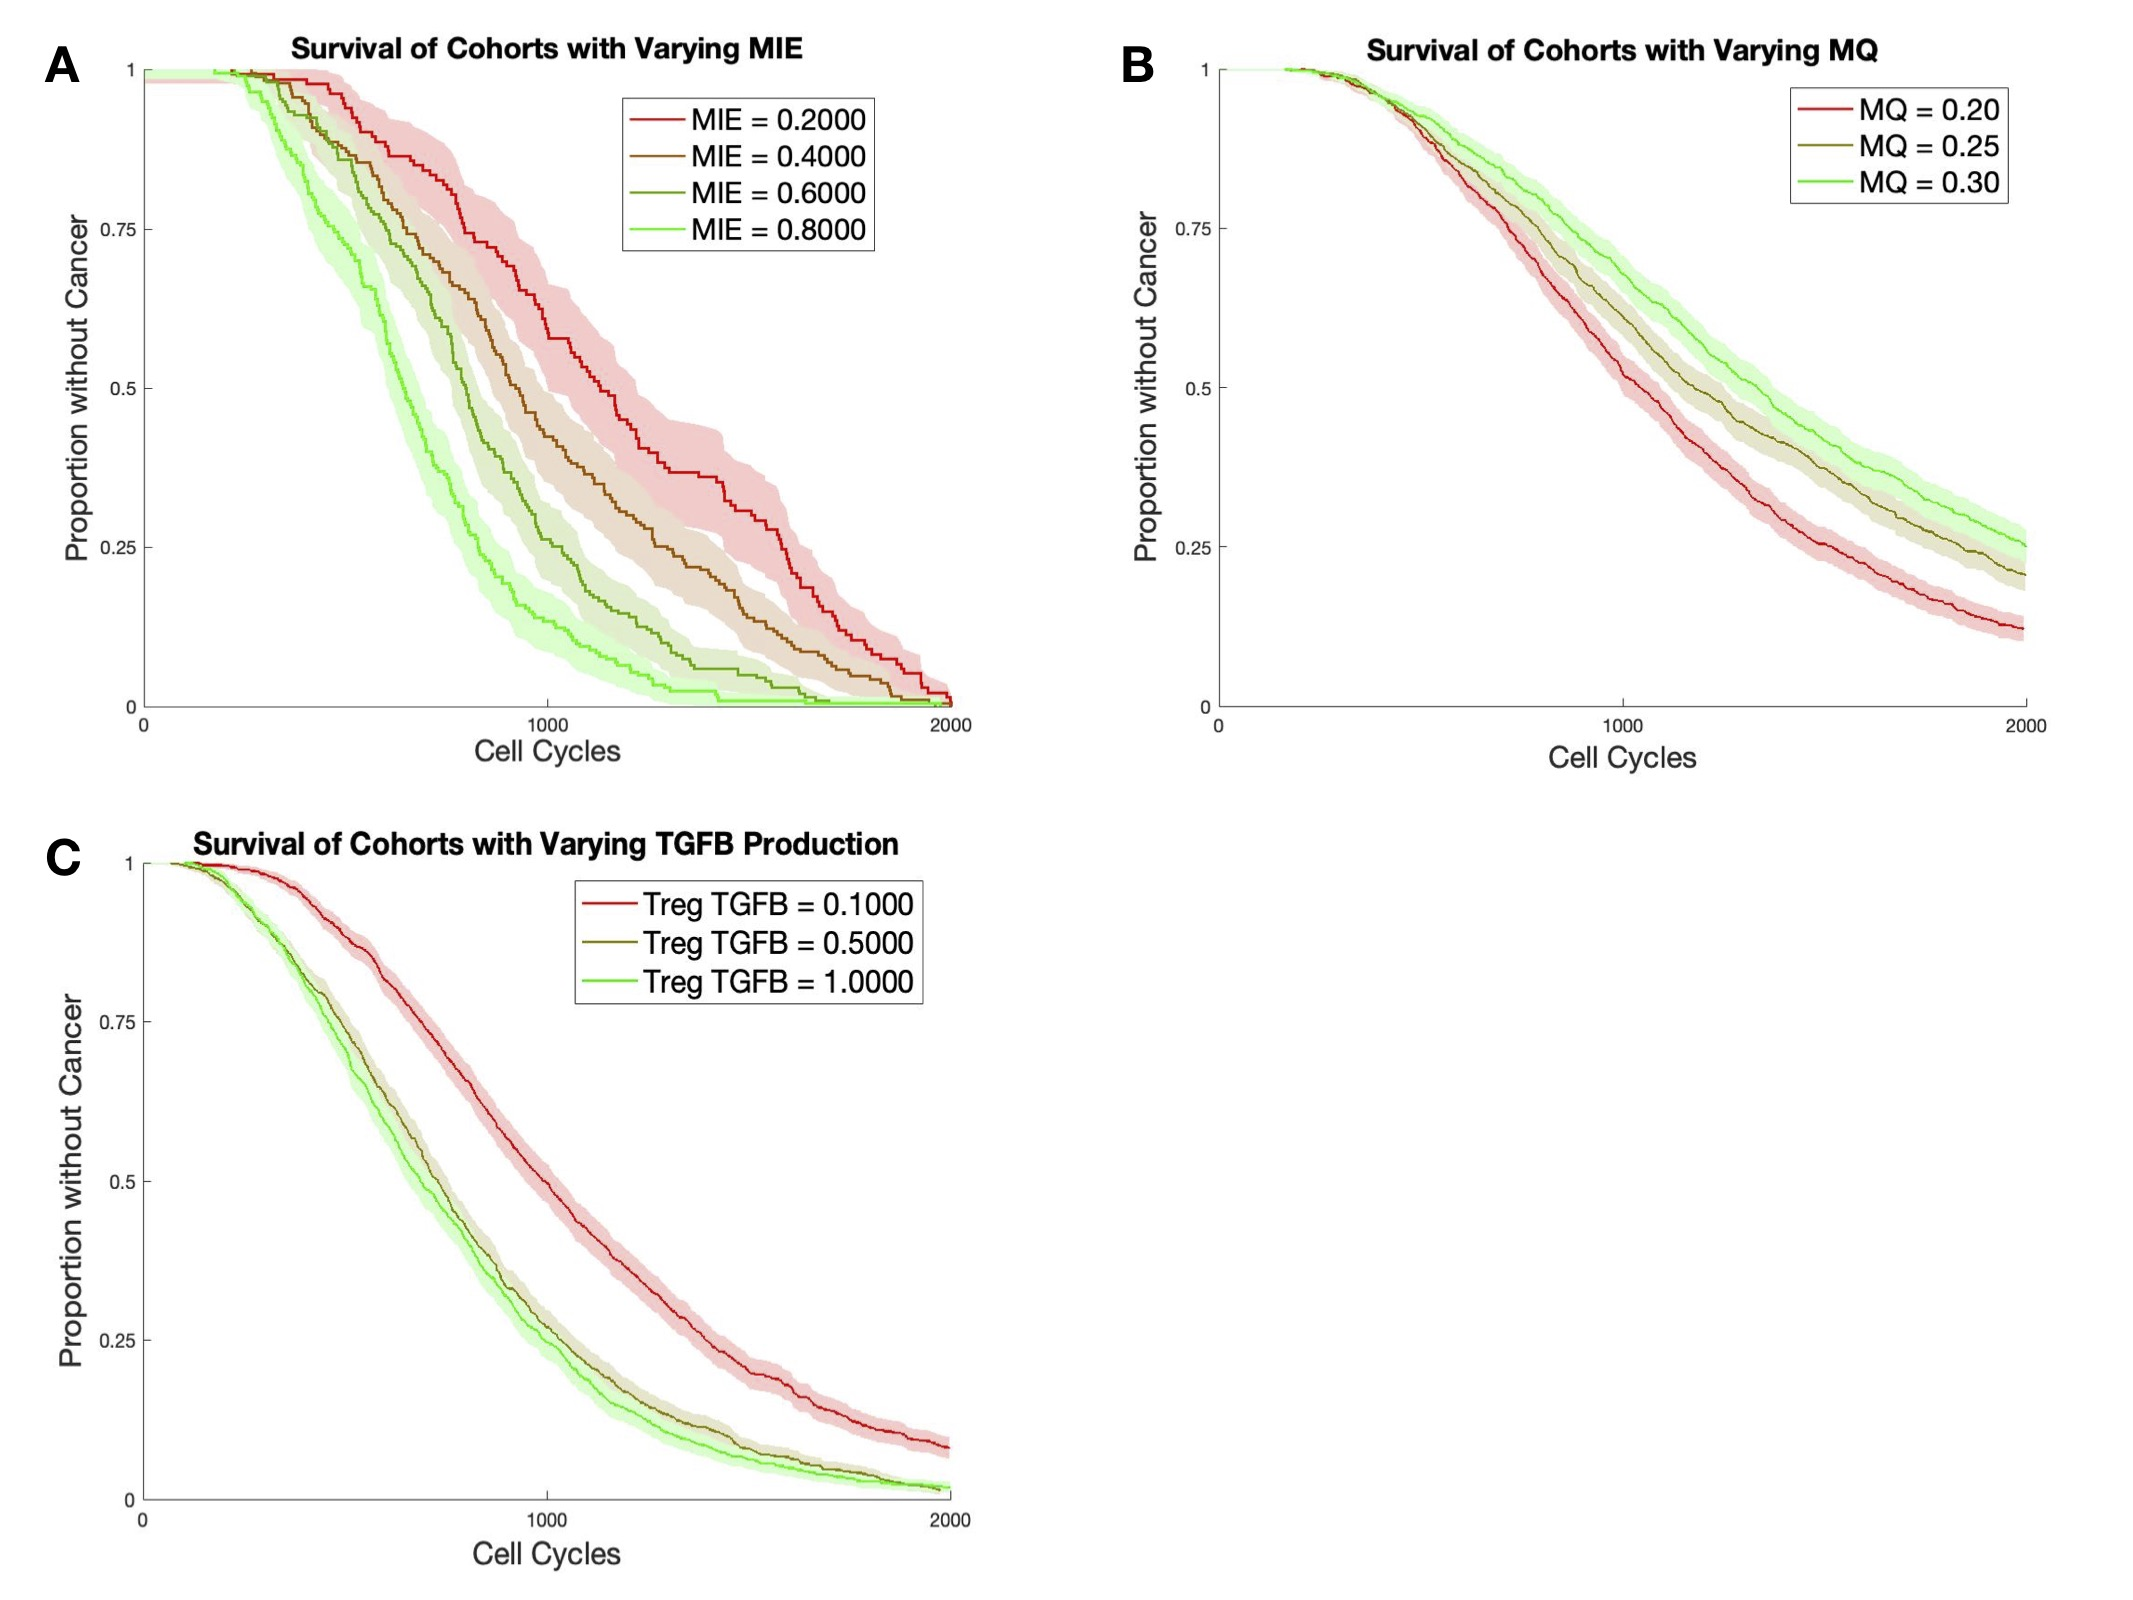
\includegraphics[width=0.85\textwidth]{Figure2/Figure2.jpg}}
\caption{Sensitivity analysis of model parameters, determined via the global Morris one-step-at-a-time method. $\mu^*$ denotes the average absolute change in Time to Cancer when the parameter is varied.}
\label{fig:MOAT}
\end{figure}

\subsection{Mesenchymal phenotypic properties dramatically change cancer-free survival times}\label{MesPars}

\begin{figure}
\center
{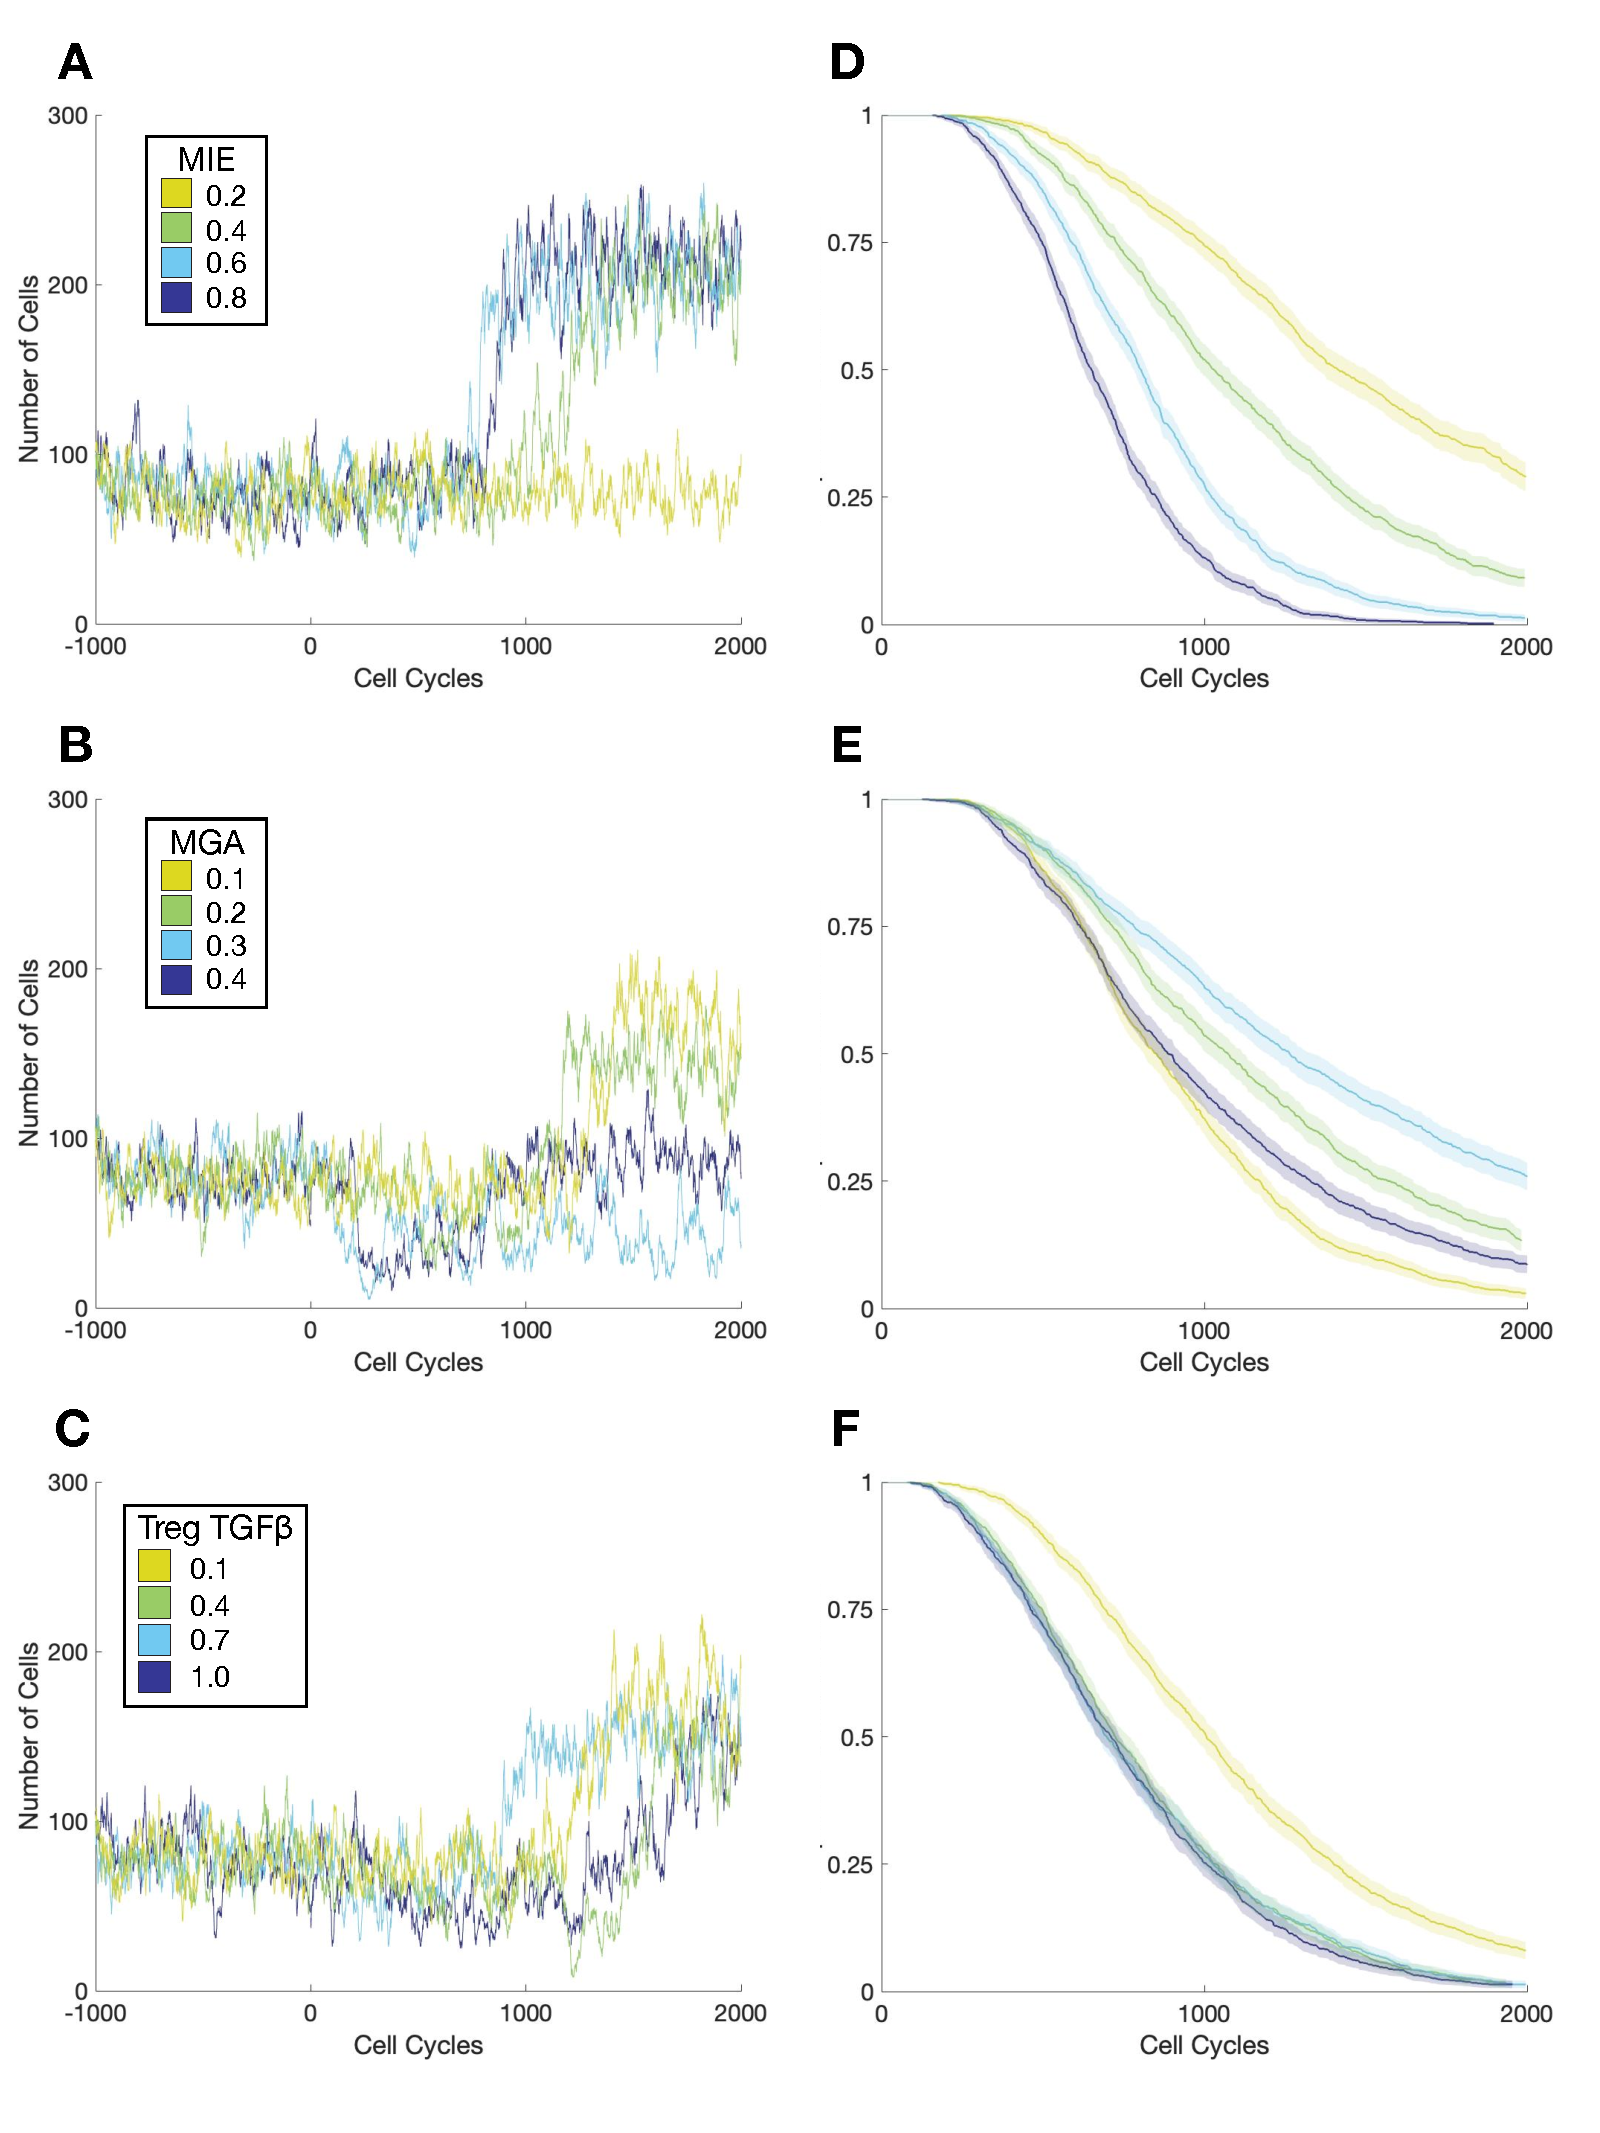
\includegraphics[width=0.85\textwidth]{Figure3/Figure3.pdf}}
\caption{Effects of mesencymal cell properites on the time to cancer. Trajectories of one patient per cohort from warmup period ([-1000,0]) to 2000 cell cycles, for $\Delta_\text{MIE}$ (A); $\Delta_\text{MGA}$ (B); and $\tau_\text{Treg}$ (C). 
D. Survival curves corresponding to changes in MIE (A) for a patient cohort of size 1000; shaded region represents the 95\% confidence interval for the evaluated function. 
E. Survival curves for patient cohort corresponding to changes in MGA (B).
F. Survival curves for patient cohort corresponding to changes in Treg TGF-$\beta$ (C). 
}
\label{fig:FirstSurvivalCurves}
\end{figure}


When a cell transitions from an epithelial to a mesenchymal state, two phenotypic cell characteristics change: mesenchymal immune evasion (MIE) and mesenchymal growth arrest (MGA).
Both parameters are defined as proportions, and lie in $[0,1]$, where higher values indicate more mesenchymal-like properties.
The parameter $\Delta_\text{MIE}$ is the proportional reduction in the probability that a \sout{mutated} \tcb{hypermutated} mesenchymal cell will be subject to immune clearance in a given cycle.
The parameter $\Delta_\text{MGA}$ is the proportional reduction in the probability that a mesenchymal cell will proliferate in a given cell cycle, thus is equivalent (strictly in terms of its impact on the cell cycle) to an increased proportion of time spent resting in the $G_0$ phase.
The cytokine TGF-$\beta$ is also involved in the EMT process (by increasing the probability of EMT). All three of these parameters were found to have large effects on the model by the Morris OAT analysis presented in Section \ref{SensAnalysis}.
\par 
As MIE is increased, the Time to Cancer decreases (Fig. \ref{fig:FirstSurvivalCurves}A) under all sets of parameters studied: as this subpopulation of \sout{potentially mutated} \tcb{hypermutated} cells becomes more resistant to immune clearance, the tumor as a whole grows more resilient and thus will grow faster.
These results are summarized by Fig. \ref{fig:FirstSurvivalCurves}A.
\par
Second, as MGA increases, Time to Cancer increases, i.e. lower proliferation rates for mesenchymal cells slow down cancer growth (Fig \ref{fig:FirstSurvivalCurves}B).
This is not immediately intuitive, since the decreased proliferation rate affects \sout{both mutated and non-mutated tissue cells.} \tcb{all mesenchymal cells, not just hypermutated cells.}
\par
Third, TGF-$\beta$ can be varied in two ways: the production by mesenchymal cells and the production by Treg cells.
In Fig \ref{fig:FirstSurvivalCurves}C, the results of varying Treg TGF-$\beta$ production are shown, indicating that an increased Treg TGF-$\beta$ production leads to a shorter Time to Cancer.
The two main ways in which TGF-$\beta$ influences the system is in recruitment of Treg cells and in pushing tissue cells to a mesenchymal phenotype.
Treg cells are modeled as tumor-protective and thus increasing their number will naturally decrease Time to Cancer.
Mesenchymal cells are more likely to evade the immune system, so pushing the system towards an overall more mesenchymal phenotype will better protect the cancer and decrease the Time to Cancer.

\begin{figure}
\center
{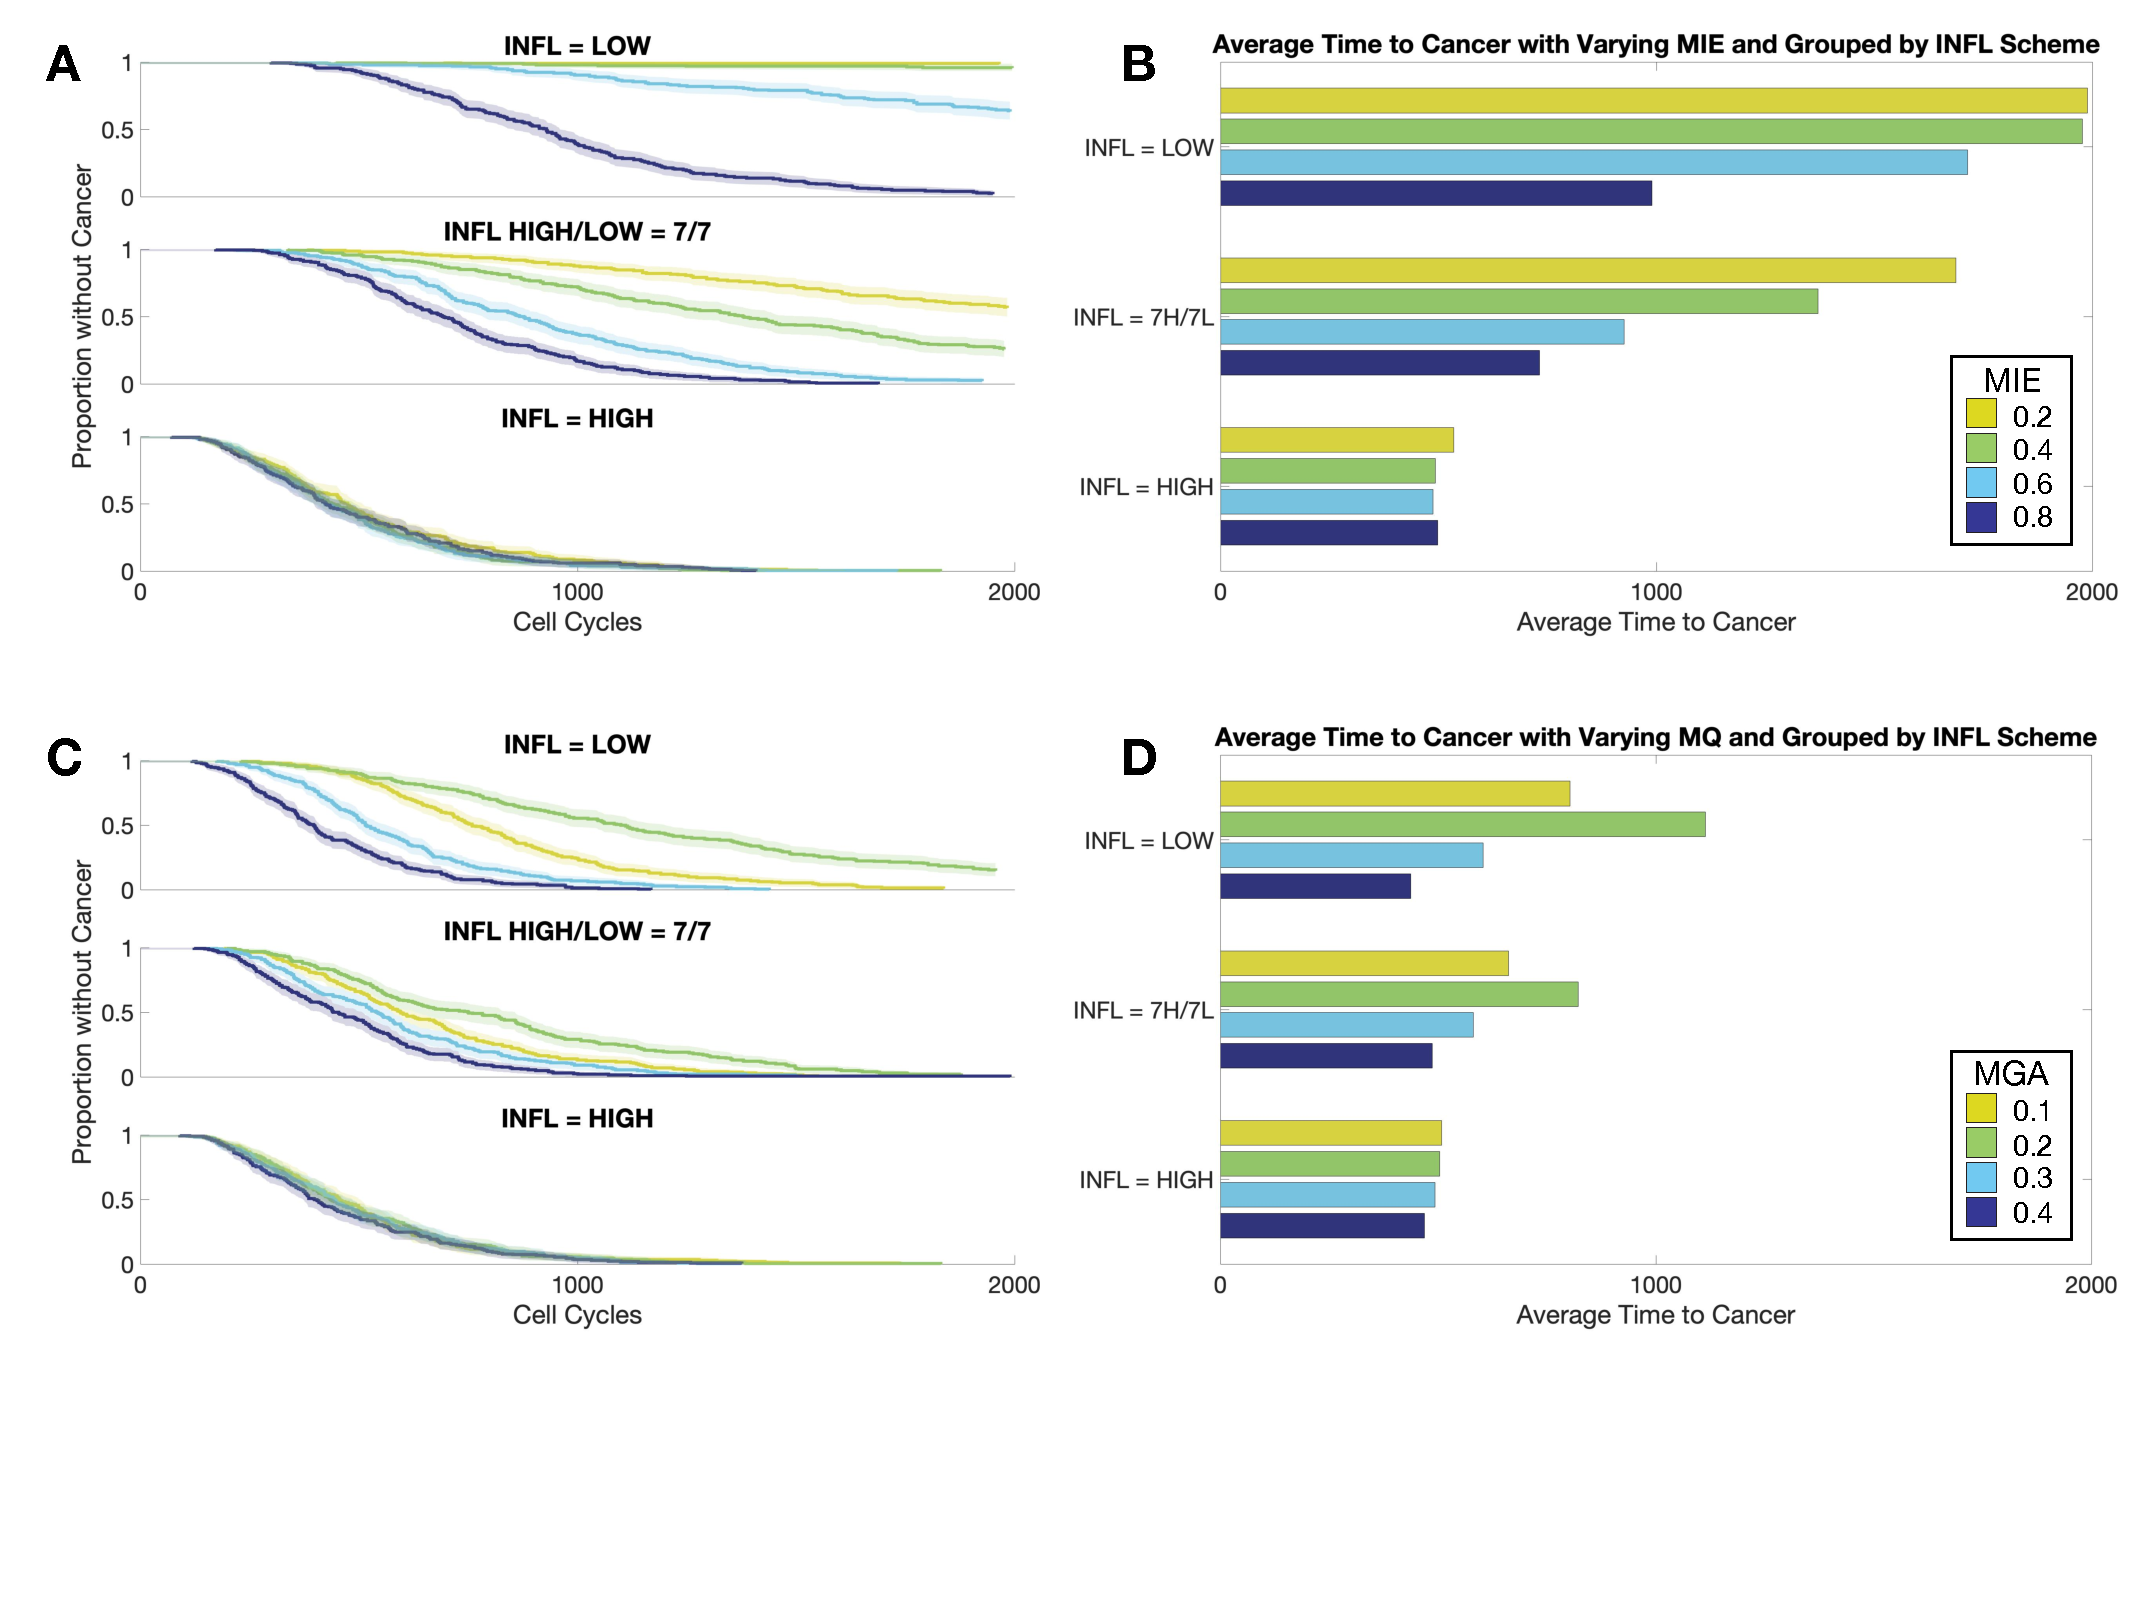
\includegraphics[width=0.95\textwidth]{Figure4/Figure4.pdf}}
\caption{Effects of inflammation on the time to cancer under different cycling schemes. A-B. As MIE varies, survival curves (each of 200 patients)  and corresponding bar plots to summarize the mean Time to Cancer for each cohort are shown. C-D. As MGA varies, survival curves  and corresponding bar plots to summarize the mean time to cancer for each cohort are shown.}
\label{fig:VaryINFL_and_MesPars}
\end{figure}

\subsection{A key EMT regime maximizes cancer-free survival time under chronic inflammation}\label{KeyEMT}

We explored the effects of varying the inflammation state of the patient on cancer-free survival, to investigate competing interactions within the TME and their effect on EMT. Patient cohorts were simulated under different inflammation regimes: permanently low inflammation; permanently high inflammation; or variable inflammation. For patients drawn from cohorts in a permanently high inflammatory state, the relationship between mesenchymal parameters and the Time to Cancer is monotonic, i.e. increasing either MIE (Fig. \ref{fig:VaryINFL_and_MesPars}A-B) or MGA (Fig. \ref{fig:VaryINFL_and_MesPars}C-D) decreases the Time to Cancer.
However, under regimes with either temporary or permanent periods of low inflammation, different relationships emerge: a local maximum for the Time to Cancer is found with respect to MGA ($\Delta_\text{MGA}= 0.3$). This is seen both for intermittent or low inflammation (Fig. \ref{fig:VaryINFL_and_MesPars}D). 
\par
These striking differences in the mean Time to Cancer -- extended by up to one \tcb{{\it in silico}} year by fine-grained optimization of mesenchymal growth arrest -- have clear therapeutic implications. 
\sout{
Our model predicts that reducing the inflammatory state of the TME in three weeks out of every nine would be provide means to prolong cancer-free survival in combination with mesenchymal cell therapies to make the control of mesenchymal proliferation an effective anti-cancer strategy.
}
\tcb{
Our model predicts that a patient suffering intermittent inflammatory attacks at the tumor site will benefit from controlling the proliferation of the mesenchymal cells.
}
\par
In contrast, when MIE is varied for different inflammation cycling schemes, regardless of the cycling scheme, increasing the MIE leads to decreases in the Time to Cancer (worse survival probabilities), although in the case where the inflammatory state is permanently high, MIE has little effect on the Time to Cancer. Thus under any inflammation regime with periods of low inflammation, any reductions in the rate of mesenchymal immune evasion will lead to improved patient outcomes.

\begin{figure}
\center
{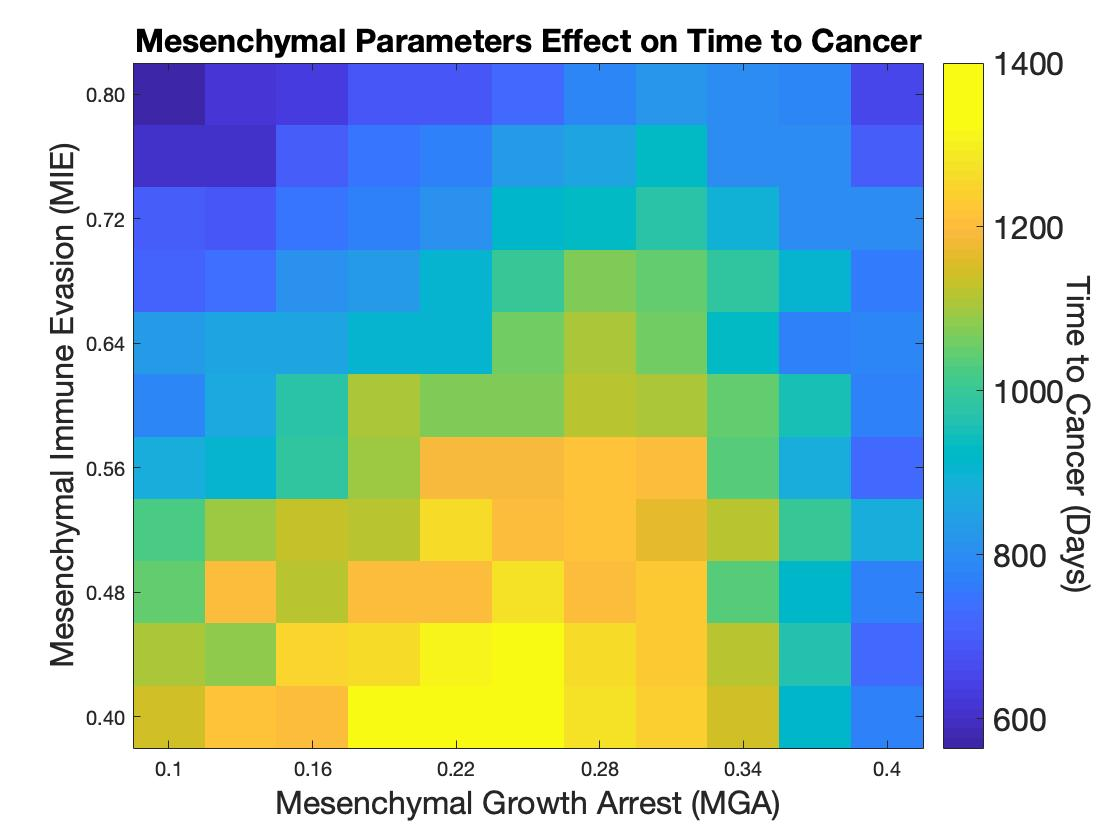
\includegraphics[width=0.5\textwidth]{Figure5/MIEvsMGA_bigcbar.jpg}}
\caption{Summary of the contrasting effects of MIE and MGA on the Time to Cancer.
}
\label{fig:MIEvsMGA}
\end{figure}

\subsection{Analysis of TCGA data in comparison with model predictions suggests that mesenchymal phenotypes reduce cancer-free survival probability}\label{tcga}


To further assess the effects on tumorigenesis of the mesenchymal properties of immune evasion and growth arrest, we study the joint density plot for each of these parameters against the Time to Cancer (Fig. \ref{fig:MIEvsMGA}). We found that over the full range of values of $\Delta_\text{MGA}$ considered, increasing $\Delta_\text{MIE}$ decreases the Time to Cancer. However, for any given value of mesenchymal immune evasion, there is a value of mesenchymal growth arrest that maximizes the Time to Cancer. Moreover, this optimal value increases with increasing MIE. Together these results show that while reducing the ability of a mutated cell to evade the immune system by any amount will improve the probability of cancer-free survival, an optimal value of MGA will prolong survival. 
\par
To compare these model predictions with experimental studies, we analyzed data from The Cancer Genome Atlas (TCGA) database to study the effects of immune and EMT interactions on prognosis of cancers for which inflammation is known to play an important role, such as colonic or pancreatic cancers \cite{greten2019inflammation,hu2010inflammation}.
We note that the comparison between simulation and data here is indirect since the model studies the progression of cancer from an arbitrary starting point, while the data address the progression of cancer following treatment, but analogous processes are at play during both the progression of  clonal dynamics addressed by the model, and the progression of disease after cancer treatment.
In particular, the plasticity of tumor cells allows them to evade treatment by undergoing post-treatment processes resembling the de-novo appearance of cancer\cite{sanchez2018slow}.
\par 
The TCGA Pan-Cancer Clinical Data Resource (TCGA-CDR) provides multiple computed clinical endpoints for PAAD \cite{liu2018integrated}.
Here, we focus on the disease-free interval (DFI) and the overall survival (OS) endpoints.
In essence, a tumor where the DFI is short will undergo rapid (post-treatment) initiation.
In turn, we expect the distance between DFI and OS to be relatively small for a tumor undergoing rapid progression following initial (post-treatment) detection.
Therefore, recurrent tumors may be roughly categorized as either rapidly progressing or slowly progressing by some arbitrary threshold of DFI/OS divergence.
We selected three tumor types whose TCGA-CDR profile indicated slow progression (OV, SKCM, LIHC) and three tumor types whose profile indicated rapid progression (PAAD, LUAD, COAD).
\par
For each cohort of cancer patients, we cluster the patients via k-means (n = 2) either on gene ontologies relating only to EMT (linked figures) or on gene ontologies relating to EMT and inflammation.  We also plot the corresponding survival curves for each of the clusters obtained (utilizing the originally reported OS endpoint). We see that in both cases, survival is affected by the gene ontology signature, but the presence of both EMT and inflammatory signatures has a greater impact on survival than the effects of EMT alone. This suggests that when studying interactions between cancer and the immune system, is it important to consider EMT; the effects of which may impact the dynamics and should not be overlooked. 

\par

\tcr{THE REST OF THIS SECTION IS FROM THE FIRST DRAFT AND WILL BE DELETED}

\par 
To compare these model predictions with experimental studies, we analyzed data from The Cancer Genome Atlas (TCGA) database to study the effects of immune and EMT interactions on prognosis of cancers for which inflammation is known to play an important role, such as colonic or pancreatic cancers \cite{hu10_inflammationinduced, balkwill01_inflammation}. Using gene ontologies as a measure of the of effects of inflammatory or EMT processes on cancer-free survival, we investigate pancreatic cancer. We note that the comparison between simulation and data here is indirect since the model studies processes occurring before incidence, while the data address subsequent events, but analogous processes are at play during both the pre-cancerous clonal dynamics addressed by the model, and the progression of disease that follows cancer incidence. 
\par
For a cohort of pancreatic cancer patients, we cluster the patients via k-means ($n=2$) either on gene ontologies relating only to EMT (Fig. \ref{fig:tcga}A) or on gene ontologies relating to EMT and inflammation (Fig. \ref{fig:tcga}C).
We also plot the corresponding survival curves for each of the clusters obtained (Fig. \ref{fig:tcga}B, D).
We see that in both cases, survival is affected by the gene ontology signature, but the presence of both EMT and inflammatory signatures has a greater impact on survival than the effects of EMT alone.
This suggests that when studying interactions between cancer and the immune system, is it important to consider EMT; the effects of which may impact the dynamics and should not be overlooked.


\begin{figure}
\center
{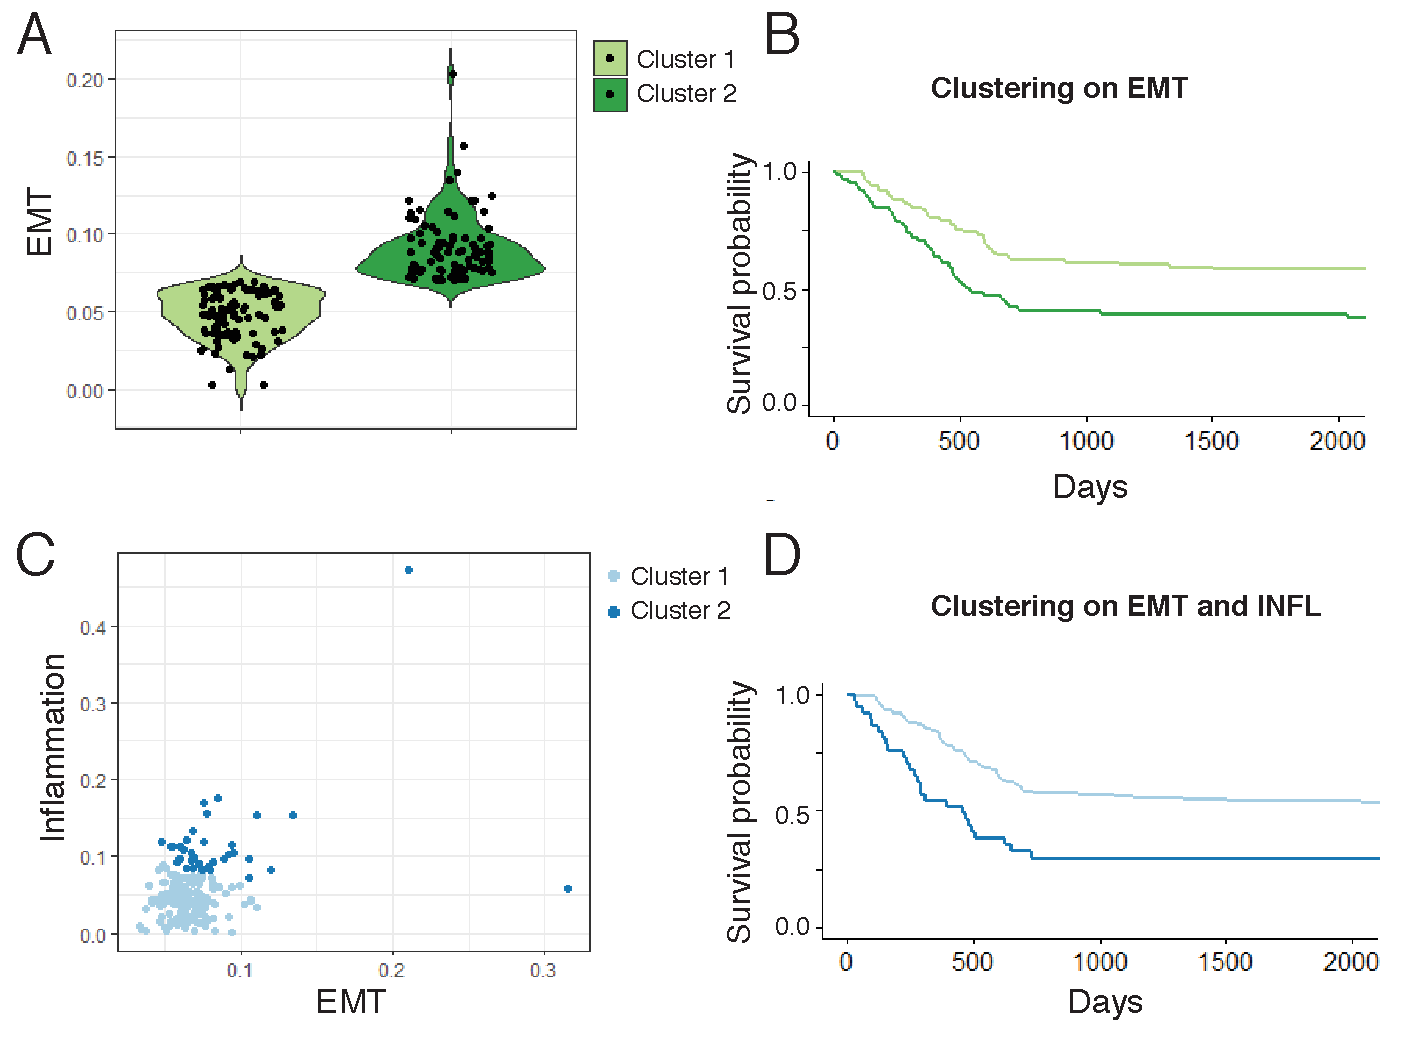
\includegraphics[width=0.9\textwidth]{FigTCGA.pdf}}
\caption{A. K-means clustering of pancreatic cancers using gene ontology terms indicative of an EMT signature ($k=2$). B. Survival plots corresponding to the clustering on EMT. C. K-means clustering of pancreatic cancers using gene ontology terms indicative of EMT and Inflammation signatures ($k=2$). D. Survival plots corresponding to the clustering on EMT and inflammation.}
\label{fig:tcga}
\end{figure}

%%%%%%%%%%%%%%%%%%%%%%%
%                      DISCUSSION                       %
%%%%%%%%%%%%%%%%%%%%%%%

\section{Discussion}\label{Discussion}
Despite the intense interest in cancer and the immune system, and in the effects of EMT on cancer, there has not previously, to the best of our knowledge, been a model developed that combines these components: cancer, the immune system, and EMT. We saw this as an even more pressing need given the shared factors that influence all of these, such as TGF-$\beta$. We used an individual cell-based model framework to describe the multiscale processes that can lead to cancer: DNA damage occurs during the cell cycle and this can lead to mutations in pathways that affect the fitness of the cell, which in turn affects the cell population dynamics, which are also influenced by the intrinsic state of the cell (EMT), and extrinsic immune factors (inflammation, cytotoxic cells, etc).
\par
We found that this model recapitulated cancer-free survival dynamics, and via global parameter sensitivity analysis, we identified parameters exerting key control over model behavior. Focusing on these led us to identify that: increasing mesenchymal immune evasion, decreasing mesenchymal growth arrest, or increasing Treg TGF-$\beta$ production all lead to shorter Times to Cancer. However varying the level of inflammation leads to paradoxical effects: under regimes with periods of low inflammation, an optimal level of mesenchymal growth arrest can improve outcomes and maximize the Time to Cancer.
\par
To test these predictions, we performed unsupervised analysis of pancreatic cancer data from The Cancer Genome Atlas, and looked at survival across two groups: we found that the presence of an EMT signature increased differences in survival between groups in combination with inflammation. We chose to summarize {\em in silico} patient simulations with a single parameter: the Time to Cancer, which we found captured the essential characteristics of the model. There are, of course, many tissue trajectories that all result in cancer, and it is our opinion that analysis of the transient cell dynamics in pre-cancerous tissues is a pressing need to shed insight into cellular biomarkers of cancer.
\par
These results represent promising steps in understanding the competing roles of the immune system and EMT during (pre-) development of epithelial cancers, yet much remains to be done. Further development of the inflammation module of this model is important given the large and sometimes paradoxical roles that the inflammatory state exerts on the epithelia and cancer-free survival (Figs. \ref{fig:MOAT} and \ref{fig:VaryINFL_and_MesPars}B, D). Currently, inflammation is modeled as independently cycling between high and low schemes, however many of the agents considered in the model actively contribute to the inflammatory state, thus it would be interesting to consider connecting these components (for example by letting the level of inflammation be conditional on the number of mutant cells in the tissue). Another layer of complexity is revealed by the natural anti-inflammatory role of Tregs. One consequence of the current model is that decreasing the number of Tregs increases the cancer-free survival. Clearly, there exists a trade-off to be accounted for, and adding to the model the main effector function of Tregs could remedy this and add depth to our understanding of the various roles that Tregs play in and around the tumor.
\par
The roles that TGF-$\beta$ plays throughout the tumor and its microenvironment also warrant further investigation. We found that, below a certain threshold, reduction of TGF-$\beta$ increases the Time to Cancer  (Fig. \ref{fig:FirstSurvivalCurves}E), thus reducing expression levels of TGF-$\beta$ in the tumor microenvironment benefits survival. Intriguingly, recent experimental work demonstrated that TGF-$\beta$ drives tumor suppression in pancreatic cancer by promoting EMT \cite{david16_tgfv}. However, TGF-$\beta$ is a master regulator implicated in numerous cellular signaling processes, and changing the concentrations of TGF-$\beta$ even in a local tumor microenvironment could have large off-target effects. Indeed, it has been showns that TGF-$\beta$ promotes invasion and heterogeneity (although suppresses cell proliferation) in squamous cell carcinoma \cite{oshimori15_tgfv}. Future work thus ought to consider the effects of targeting signaling factors downstream of TGF-$\beta$ that still have the ability to modulate epithelial cell dynamics. Towards this end, we are currently developing a larger TGF-$\beta$ signaling pathway module with appropriate crosstalks to  epithelial/mesenchymal/immune cell functions to be incorporated into the model.
\par
A further goal for future work is to explore (and exploit) the heterogeneity of tumor evolution in greater depth: this heterogeneity aids the evasion of the tumor from immune effects. Studying the consequences of decanalization \cite{gibson09_decanalization} during cancer progression is too-often sidelined, despite evidence supporting its prominence \cite{cyll17_tumour, punt17_tumour, dagogo-jack18_tumour}. Yet despite these challenges, for which the complexity of the disease may be often in large part responsible, great progress has been and continues to be made. As we approach a new generation of immunotherapies, it is these very complexities that we must better understand in order to control or eradicate the disease.

\section*{Acknowledgements}
The work is partially supported by National Institutes of Health grants R01GM123731, U01AR073159, and U54-CA217378; National Science Foundation grants DMS1562176 and DMS1763272; The Simons Foundation grant (594598 to Q.N.) and a grant from the Jayne Koskinas Ted Giovanis Foundation for Health and Policy joint with the Breast Cancer Research Foundation.


\bibliography{mybib,amrefs}
\bibliographystyle{plos2015}

\end{document}